\documentclass[a4paper, 12pt]{article} 
\setlength{\parindent}{0em}
\usepackage[margin=0.8in]{geometry}
\usepackage{tabularx}
\setlength{\parskip}{1em}
\usepackage{graphicx}
\graphicspath{C:/Users/Zola South/Documents/School stuff/COMS Assignment/Proposal}
%%\usepackage{subfigure}
\usepackage[labelsep=endash]{caption}
%\usepackage{subcaption}
\usepackage[section]{placeins}
\usepackage{float}


\title{\textbf{UniNceda}}
\author{Group 45 \\ \\ Sibongakonke Kubheka (1933028)\\ Ureeshah Moodley (1600076) \\ Siphesihle Mthethwa (2093411) \\ Nomfundo Luthuli (2208451) \\ Makoko Campbell Manape (2127079) \\ Thabang Tshikwatamba (1881518)}
\date{\today}



\begin{document}

{\let\newpage\relax\maketitle}
\textbf{\large{Division of Labour}}
\newline
\newline

\begin{tabularx}{\textwidth}{llX}
\hline
%\vspace{5pt}
\# & Name & Description \\
\hline
1 & S. Kubheka & Work with 2 and 3 to identify the scope of the project, the current systems and describe the proposed system. Gather data to elicit requirements through brainstorming sessions with assistance from 3.\\
2 & U. Moodley & Work with 1 and 3 to identify the scope of the project, the current systems and describe the proposed system. Gather data to elicit requirements through interviews with assistance from 6.\\
3 & N. Luthuli & Work with 1 and 2 to identify the scope of the project, the current systems and describe the proposed system.\\
4 & S. Mthethwa & Work with 5 and 6 to formulate the functional requirements, the non-functional requirements and design the system models for the proposed system. Gather data to elicit requirements by synthesising the requirements from existing systems with assistance from 6.\\
5 & T. Tshikwatamba & Work with 4 and 6 to formulate the functional requirements, the non-functional requirements and design the system models for the proposed system.\\
6 & M.C. Manape & Work with 4 and 5 to formulate the functional requirements, the non-functional requirements and design the system models for the proposed system.\\
\hline
\end{tabularx}

\newpage

\tableofcontents
\pagenumbering{arabic}
\newpage
\pagenumbering{arabic}

\section{Introduction}
(First Year Assistance) is an application which is intended to become a centralized service that students use to apply to any local public university – specifically to a point where in the near future, anyone (matric or older) who would like to study an undergraduate degree in South Africa will have to apply through this application/service. 


According to a report by Inside Education, more than \textbf{40 percent} of first-year students have dropped out of university since the independence of South Africa. A significant percent of this is due to students feeling as though they have made both the wrong degree and career choice. This could be due to a lack of career guidance in schools and general pressures on the matric/prospective student. Dropping out of university can not only be stressful for students, but also costly for both the family and the university. Thus the intended purpose of this project is to help eliminate one of the many reasons why students drop out of university.

With the application successfully implemented, the app will assist in providing tailored information, regarding all public universities in South Africa, to the student.

\subsection{Scope} 
Ultimately the app looks to make the application process as stress free and as easy as possible, leaving the students informed and with access to the necessary resources. The main aim of the application is to equip prospective students to make better informed decisions about their university degrees as well as reduce the stress that comes along with application process. 

Each student will have to create a profile within the app. This will require personal information as well as results from school, their preferred degree choices, monthly household income etc. This will tailor the information according to their abilities, preferences and circumstances, allowing students to be able to choose the degree that not only suits their interests and passion, but also suits their marks.

The information covered will be general information regarding the universities, the respective degrees offered, the application process, and information regarding both financial aid and student accommodation.

Currently, necessary information such as course outlines and what specific degrees actually entail are a scarce resource. Students are required to perform their own research in many different forms and for some this is not necessarily an easy task to do. With the app, we will ultimately simplify the application process for all prospective students.

\subsection{Definitions and Conventions}

Administrator: team behind the app that collects and stores the apps information for the users. They then update and maintain the system ensuring all information is correct and up to date.

App: an application, especially as downloaded by a user to a mobile device

Personal statement: a written description of one's achievements, interests, etc., included as part of an application for a job or a place at university or college.

User: any person(s) looking to study at a public university in South Africa for the first time.

UCAS: Universities and Colleges Admissions Service

UK: United Kingdom 


\subsection{Overview}

The following document is a walk through of the proposed application/website.

It covers the following:
\begin{itemize}
\item Any similar existing systems and how the proposed idea is better 
\item How the app will work, as well as its pros and cons
\item The proposed system
\item The requirements as set by the proposed user 
\item Functional requirements 
\item Non-functional requirements 
\item System Models
\end{itemize}

\newpage
\section{Current Systems}

\begin{itemize}
\item UCAS \\

UCAS is a online admissions portal service that is only offered in the United Kingdom, and is a service that requires the user to pay a specific fee. For a single application it costs 18 euros and for multiple applications it costs 24 euros. The service specifically aids undergraduates with their applications for universities within the United Kingdom, as well as offer services for postgraduates and teachers.

The current UCAS system helps prospective students with the following:

\begin{itemize}
\item Filling out the application and tracking it once it has been sent in 
\item The service helps the student with their personal statements. .
\item The service further aids students in getting references to help the applicant stand out.
\end{itemize}

However, some of the downsides to this service include the fact that:

\begin{itemize}
\item It is not free, unlike what we propose for our website/app.
\item Their service is very limited and does not cover as much information we propose to cover.
\item Their information is very general and not tailored for each student. 
\item Limited to universities in the UK
\end{itemize}


(https://www.ucas.com/ - reference) \\

\item CommonApp \\

Another present system currently in use is the CommonApp. The CommonApp is another undergraduate college admissions application that applicants may use to apply to more than 800 colleges and universities in the US, Columbia, Canada, China and many other European countries. Its mission is to "promote access, equity and integrity" in the college admission process, which includes subjective factors such as essays and recommendations alongside other objective criteria such as class rank. The CommonApp further allows applicants to self-report standardized test scores and international educational qualifications. \\

One of the biggest limitations of this existing system, again, is the limited range in terms of which countries are able to use and implement this system. 

\end{itemize}

Here in South Africa there currently is no similar system in place. Prospective students looking to study here in South Africa have to work with are all the separate websites and emails that correspond to each university and/or financial aid.

Our proposed system looks to collect all the above information and much more, and tailors it to each individual student according to their registered profile. The proposed system looks to help students looking to study in any public South African university, and further takes the current application proceedings and makes it more efficient and less demanding of the user.


\newpage
\section{Proposed System}

The following section will discuss in detail how the proposed app/website will work.

\subsection{Product Perspective and Functions and User Characteristics}

User perspective: there will be a system in place in the form of an app or a website for prospective students to access information regarding them, during their application process to public South African universities. 

All students are required to register an account providing us with all the necessary information to tailor the vast amount of information to them. As mentioned before the app is profile based and therefore will be presented to them as such. In each user’s profile will be all the information regarding them separated into different categories. Students will be able to edit their profile information but nothing else. They would not have the permissions necessary to modify any information that other users have access too.

Example:

User A wants to study law, specifically an LLB. They have an A aggregate and are looking to stay in a university residence.
The basic categories on User A’s profile will be:

\textbf{Account:}
\begin{itemize}
\item Personal information - name, residence etc.
\item Academic transcripts - matric marks and/or any previous tertiary education results
\item Financial information - i.e. monthly household income 
\end{itemize}

\textbf{Applications:}
\begin{itemize}
\item Closing dates
\item Application help 
\item General information 
\end{itemize}

\textbf{Course information:}
\begin{itemize}
\item Course outline - in this case a breakdown of the LLB course.
\item Requirements - current available marks, final matric marks, APS and age exemption explained 
\item Careers - what can the student do with their degree?
\item Curriculum - modules, credits explained, prerequisites etc.
\end{itemize}

\textbf{Fees and Funding:}
\begin{itemize}
\item Estimated first year costs - tuition, text books.
\item Residence costs - food and accommodation
\item Bursaries and scholarships  
\end{itemize}

\textbf{Residence:} 
\begin{itemize}
\item Different residences within each university 
\item Entrance requirements for each residence and the requirements to remain in the residence 
\item Brief explanation of res life.
\end{itemize}

Administration perspective: this would be a separate server where admin can modify and update the information provided to the user. Admin would have their own accounts and login information. They can modify the information provided however they do not personally have access to student’s personal information as this will be kept private and is merely used to filter information.


\subsection{Constraints and Assumptions}

One big constraint includes the fact that the user and admin will require access to a mobile device in which they can use the app or webite.

Additionally, for the proposed app/website to work, an active internet connection is required. The average webpage uses around 3MB to load and will download in seconds. Due to the apps’ very basic functionality, if the user is able to load a webpage, their internet speed will be good enough to run the app. Hence a basic 3 Mbps download and 1.5 Mbps upload should be sufficient. 

The app will have to ask permission to access files on whatever device the user accesses it from. This is due to needing verified academic transcripts from the user in order to complete their profile. 

The app will not require GPS to track the user’s location as it is not necessary for any functionality within the app. Nor will it require access to the camera or microphone.  
 
\newpage
\section{Requirements Elicitation}

The brainstorming session yielded the following basic points: 

\begin{itemize}
\item Connect students to the universities
\item Help inform students about degrees, courses, scholarships etc.
\item The app should be account based/personal to the user 
\item Account should include personal information, results and financial status
\item Results of the account information filters information 
\item Detailed explanations on courses.
\item Calculate APS 
\item Notifies user of the deadline for applications(academic and financial)
\item Local public universities - start small
\end{itemize}

\textbf{Online survey:}

To obtain alternative perspectives we set up an online survey using Survey Monkey to get feedback from prospective students - our target market.

The questions were as follows:

\begin{itemize}
\item Please enter your name. (Optional question)
\item Have you applied for university? 
\item If yes for Q2, how did you find the application process?
\item Does the proposed app sound useful?
\item Do you feel you have/had all the information that you personally needed for tertiary education during the application process? i.e course outlines, degree descriptions, fees, payment options etc.
\item If you like the idea of the above app, what functionalities would you recommend we included? In other words, what information would like to be included?
\item In order for the information to be personalized, the app requires input from the user. This would be in the form of setting up an account and inputting information such as personal information, academic record and household income. Would you be fine with this? Everything would be kept private
\item Lastly would a public chatroom within the app interest you? This would be to connect to other prospective students
\end{itemize}

\newpage
The results of the conducted survey were as follows 

\underline{Question 1:} answers for this question were not relevant to the functionality study 

\underline{Question 2}: 
\begin{figure}[h]
\centering
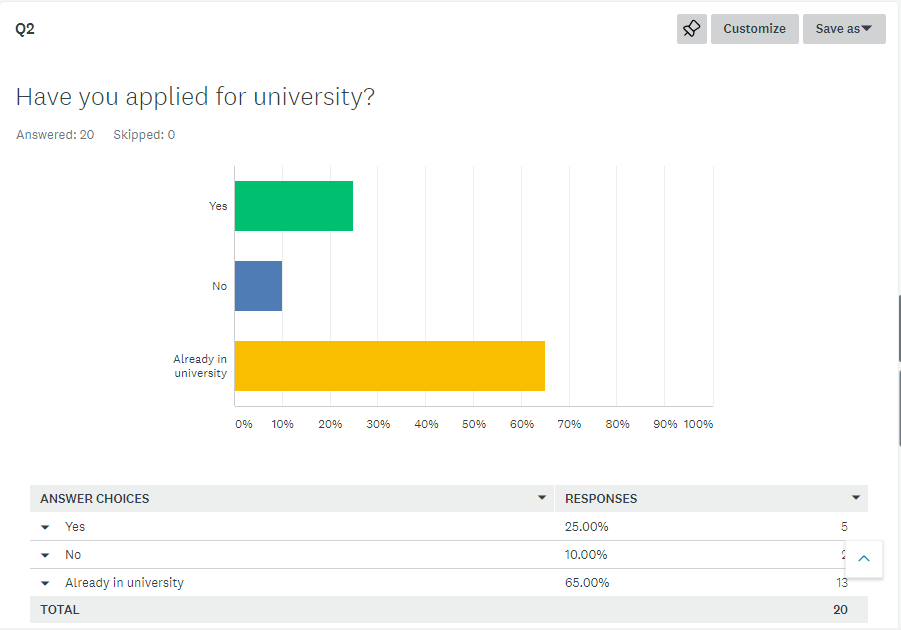
\includegraphics[scale=0.6]{Q2}
\caption{Percentage of students that have applied for university}
\label{fig: 1}
\end{figure}

\newpage
\underline{Question 3}:

\begin{figure}[h]
\centering
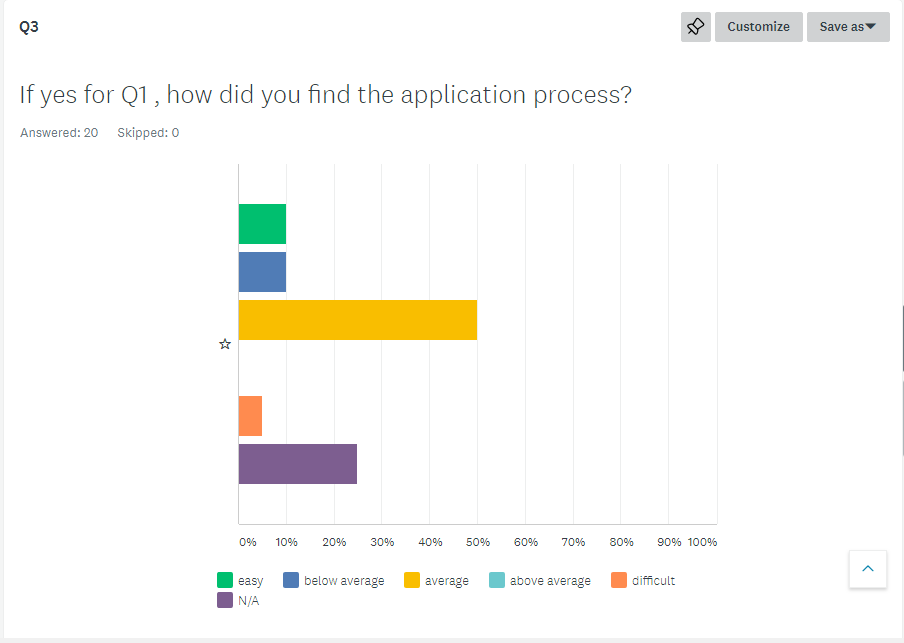
\includegraphics[scale=0.6]{Q3}
\caption{Percentage of the applicants that found the application process}
\label{fig:2}
\end{figure}

\newpage
\underline{Question 4}:

\begin{figure}[h]
\centering
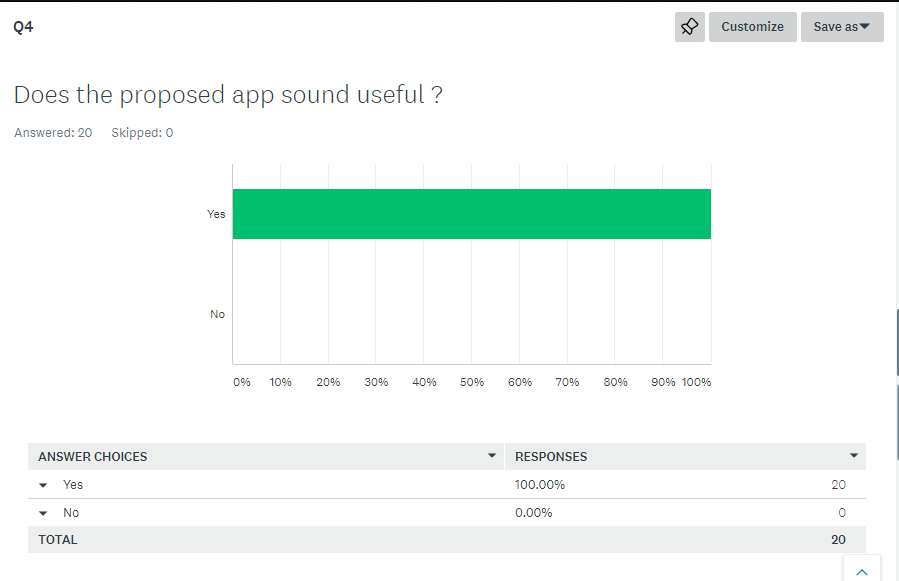
\includegraphics[scale=0.6]{Q4}
\caption{Percentage of students who found the proposed system useful}
\label{fig:3}
\end{figure}

\newpage
\underline{Question 5}:

\begin{figure}[h]
\centering
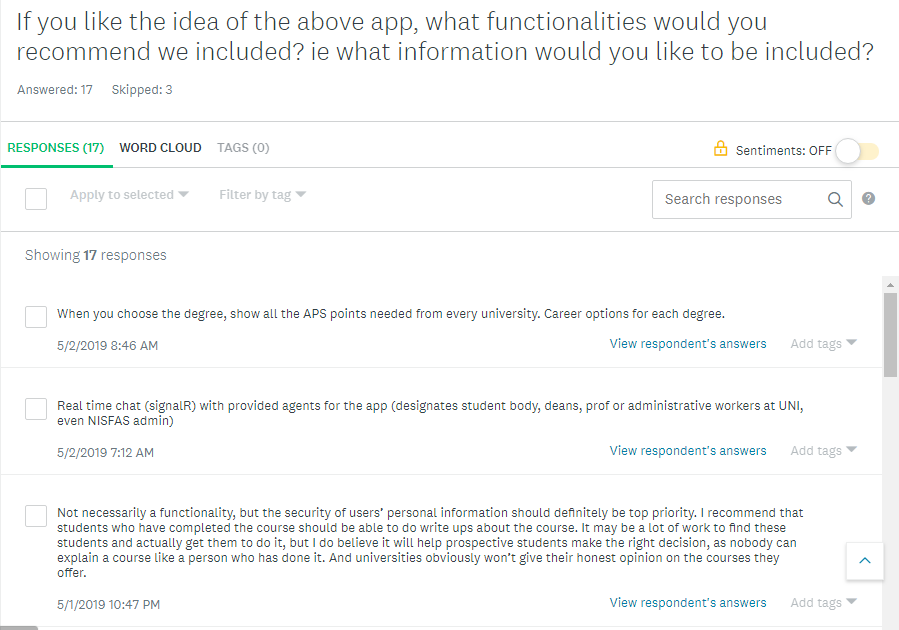
\includegraphics[scale=0.6]{Q5}
\caption{Percentage of students who felt they had all the necessary information when applying}
\label{fig:4}
\end{figure}

\newpage
\underline{Question 6}:

\begin{figure}[h]
\centering
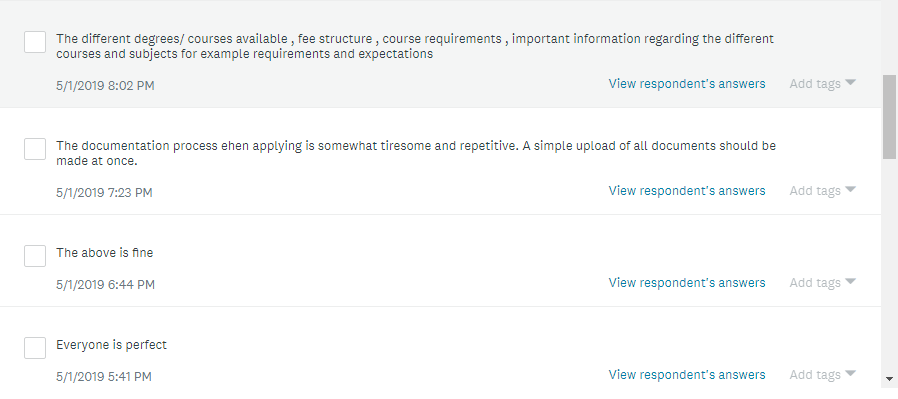
\includegraphics[width=\linewidth]{Q6}
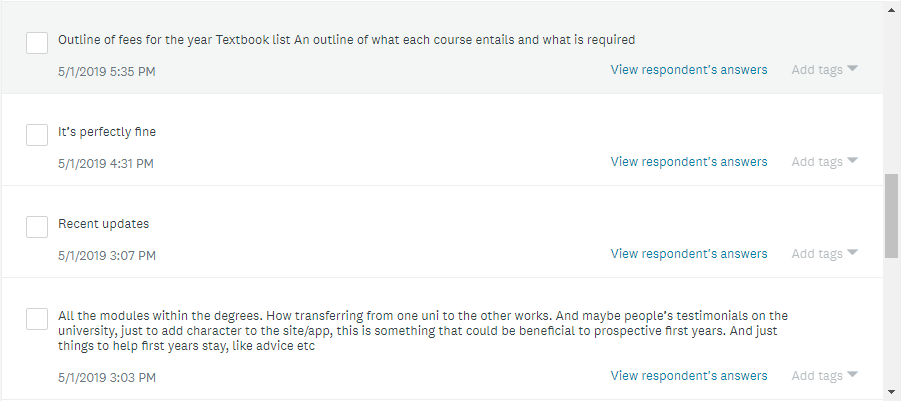
\includegraphics[width=\linewidth]{Q6_2}
\caption{Responses to what students would like to see be included}
\label{fig:5}
\end{figure}

\newpage
\underline{Question 6 (continued)}:

\begin{figure}[h]
\centering
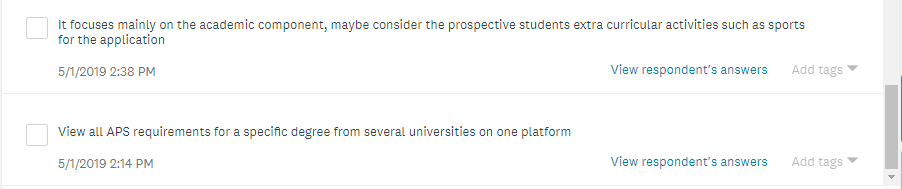
\includegraphics[width=\linewidth]{Q6_3}
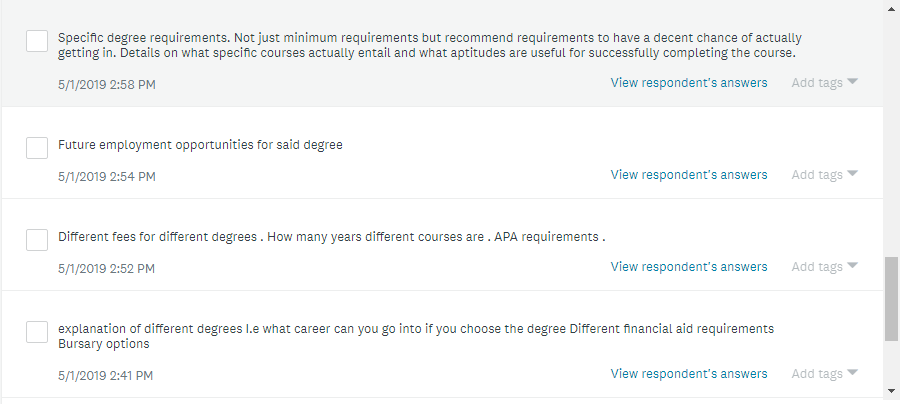
\includegraphics[width=\linewidth]{Q6_4}
\caption{Responses to what students would like to see be included}
\label{fig:5}
\end{figure}

\newpage
\underline{Question 7}:

\begin{figure}[h]
\centering
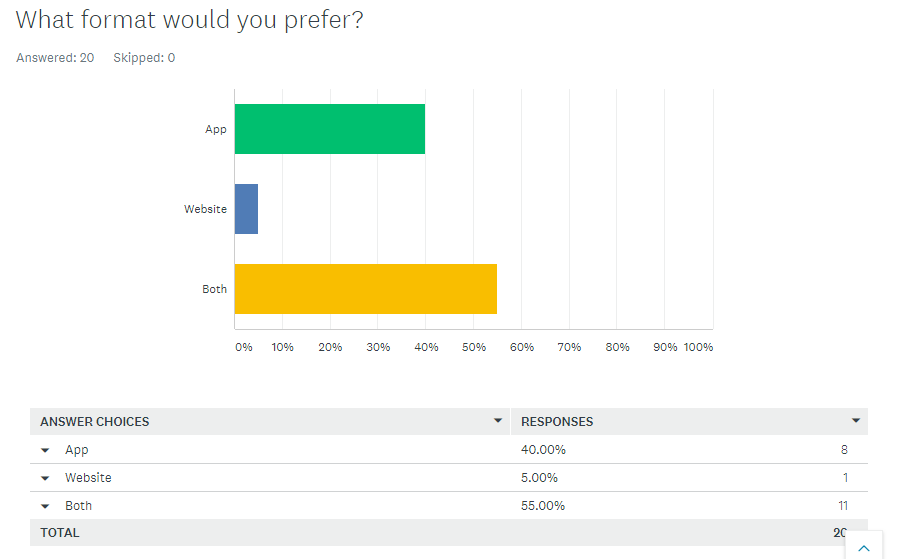
\includegraphics[scale=0.6]{Q7}
\caption{Format preference}
\label{fig:6}
\end{figure}

\newpage
\underline{Question 8}:

\begin{figure}[h]
\centering
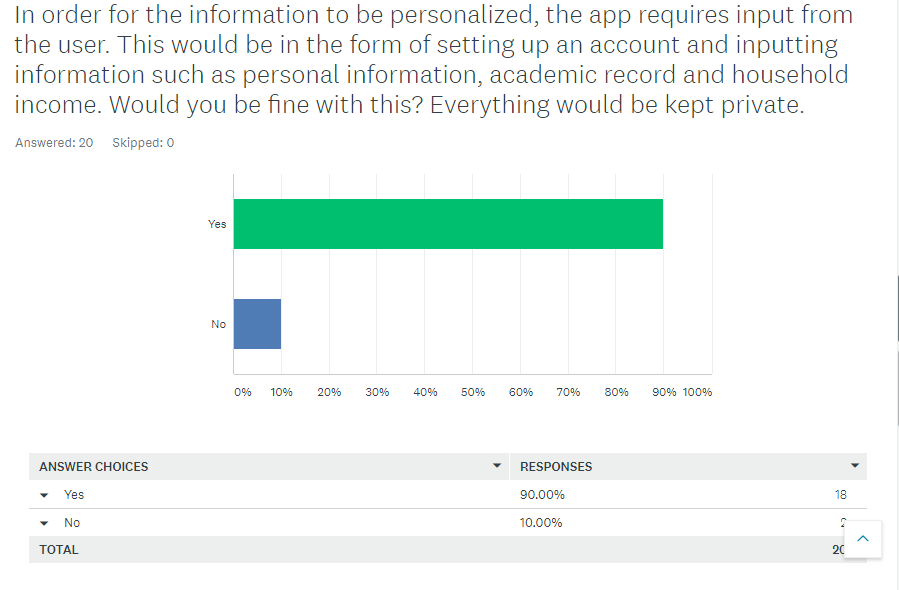
\includegraphics[scale=0.6]{Q8}
\caption{Percentage of students who would be fine with the app accessing personal information}
\label{fig:7}
\end{figure}

\newpage
\underline{Question 9}:

\begin{figure}[h]
\centering
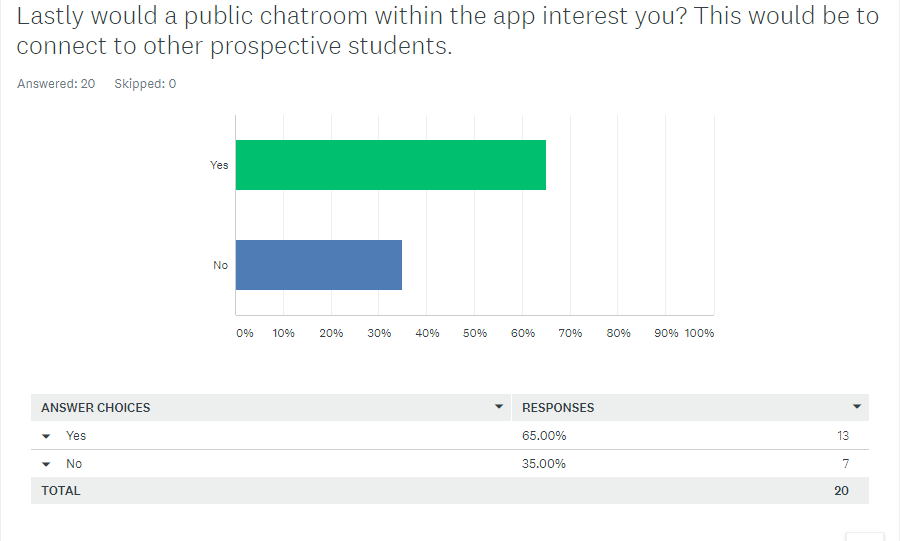
\includegraphics[scale=0.6]{Q9}
\caption{Percentage of students who would like the idea of a potential public chatroom within the app}
\label{fig:8}
\end{figure} 

\newpage
\textbf{Synthesizing the requirements from existing systems}

From the existing systems which were identified earlier in the document, the following requirements were extracted:

A.  User requirements 
\begin{itemize}
\item Enable the user to search or query information about their degree of choice.
\item Connect the users to the university officials and current students of the universities in order for them to ask questions about the university experience and find out more about the university.
\item Offer career guidance to users by providing information about the different types of careers they can pursue and the study requirements based on their profile.
\item Provide information about open days and enable the  users to book tours.
\item Initiate the application for the users by sending all the information in their profile to the university application systems. This will allow the users to apply to more than one university simultaneously 
\end{itemize}

These requirements were firstly extracted from the conducted survey in which students of varying age participated in. Furthermore, gathering information about these university application systems from various websites, as well as exploring the comments and reviews made from people who used the system before, we were able to extract these requirements.Through this method the inner workings of the systems were made visible

\newpage
\section{Functional Requirements}
\subsection{User Class}

\subsubsection{Downloading the Application}

The website will be available and accessible on the internet (e.g. Google chrome browsers) for laptops, desktops and mobile devices.
Therefore, to access the website the user only needs to download a web browser.

\subsubsection{Registration}

Each user will be required to enter his or her own personal details about themselves in order to generate their profile. 
This personal information would include name, address, phone number, and email address.

For the user to register, they would need to have working email address. This is for the purpose of active communication and so that the user is able to be reached. Furthermore, the user will need to create their own unique username and will be required to create a password for his/her account.

The following will be shown on the website before a successful login or creation of an account:

\begin{itemize}
\item Do you already have an existing account? If yes, go to LOGIN button. If not, create a new account.
\item If user has an existing account: Username and Password required.
\item If the user chooses to create a new account, the first steps, asking for the users personal details such as name, surname, age etc. will be asked
\item Next: Create a username by entering your email address
\item Create a password (must include upper and lower case characters, and a number or special character)
\item A confirmation email with an activation link will be sent to the user's address once the user has clicked confirm.
\item Once account activated: You have successfully activated your account will be displayed on the website.
\end{itemize}

Following on from an activation email being sent, the user will be given one day to activate the account before having to re-complete the process.

If the user enters an incorrect email address or password when logging in, the website will automatically inform the user that the username or password is incorrect. In the event that this occurs, the website will further indicate red colours to the both of the relevant blocks.

In the event that the user inputs and existing username when registering, the website will automatically inform the user about this. 

If all the details are correct it will submit all this information to the administrator and a message will automatically be displayed on the screen saying that an email, with a link to sign into to the website, has been sent to the user. 

\subsubsection{Forgot Password}

There will be an option on the home screen which asks the user if he or she has forgotten their password. If this is the case, the user will have to:

\begin{itemize}
\item Re-enter their email address and click enter
\item An email with a link to reset the password will be sent to the respective email address
\end{itemize}

\subsubsection{Intuitive and Easy Navigation}

Note that intuitive navigation and overall usability are the key functions our users need in our website. Minimizing clicks and actions is a good idea of increasing the website experience. Without the use of a mouse and a keyboard, it’s more difficult to select objects and input information on the website. 

\subsubsection{A Rich Experience}

Our website is going to be accessed frequently by users and we offer some experience that is not available elsewhere.

\subsubsection{Seamless Checkout}

Our website will have small touches that makes the process faster and easier for users. As with other areas of our website, fields and buttons are optimized to be easily selected.

\subsubsection{Personalized Experiences}

Website personalization can be achieved based on factors such as demographics, actions that users take in the website and the user’s current location. 

\subsubsection{Instant Query Results}

Such a feature will enable the user view the search results instantly for each character he/she types into the search bar as opposed to typing the whole search key and then waiting for the results to appear. 

\subsubsection{Real-Time Communication with university officials}

This feature enables the user to communicate through an interactive chatbox with the university officials to find out more information about that university. This is real time communication and so there are no delays in receiving messages.

\subsubsection{Viewing and Editing Account Information}

With this feature, the user will be able to view his/her account information and edit it through the button controls and inputting information in the corresponding text fields.

\subsubsection{Receiving Notifications}

This feature enables the user to receive notifications from the universities about the application deadlines and any other relevant information. This is achieved through an inbox containing a message list.

\subsubsection{Building a Profile}

\underline{Save Current Progress}

By clicking the save button the user will be able to save the current progress of filling in the application information into the forms. The user can then return to the form at a later stage and continue with the process.

\underline{Automatic Redirection}

When the user clicks the submit button on any form, the website will automatically redirect the user to the next page (according to the flow of the website).

\underline{Form Validation}

When the user clicks the submit button on any form, the website will perform validation on the data inputted into the form. This is to ensure that only valid and error-free data is stored in the database.

\underline{Fee estimator}

This feature enables the user to get an estimate of the first year university fees based on the parameters the user provides, these include the course, the funding type and the university.

\underline{Document uploader}

This feature enables the user to upload the required documents into the website, selecting the document from local storage. It also enables the user to remove an uploaded document.

\subsection{Administrative Class}

This will include everyone who will be training users, making troubleshoots, performing diagnosis, maintaining the website etc. 


\subsubsection{Admin Information device}

This class is used to specify meta information of a device administrator component. They also enforces remote/local device security policies.

\subsubsection{Admin receiver device}

This ensure that only the system can interact with the receiver (no other service can be granted this permission). This prevents other services from abusing the admininstrator's device.

\subsubsection{DNS server log service}

This allows the administrator to view the current logs of the website from their own devices. This will keep the administrator up to date about the state of the website.

\subsubsection{Viewing the metrics of the website}

This will allow the administrator to view the traffic that the website has, the throughput rate, and many more metrics. The administrator will be able to view this data in a graph, this is to ensure easy interpretation of information.

\subsubsection{Unique login portal}

The administrators will have their own secure login portal, unique from the login portal for the users. They can access this portal from the original website but through a different port.

\subsubsection{Dashboard}

The administrators can access this service via their login portal. The dashboard is a very useful tool in that it enables the administrators to edit the website content and also view the website metrics.

\newpage
\section{Non-functional Requirements}


\subsection{Reliability}

The reliability of the website could prove to be essential in terms of introducing and implementing this system nationwide. One of the most important things for a website like ours to be reliable is stability and security. This essentially means that the functionality of the website would need to experience a limited amount of errors that may disturb or hinder our users from using the website. Additionally, it would mean that the website would need to be able to safely secure the personal information provided by the user, to a point where only the user and the intended university can access this information. (Admin maybe?)

If the website was to not respond, it could cause added frustration and stress in the users who may end up resorting to previous methods. Furthermore, in entering one's personal information such as marks, the user trusts the website to keep this information safe. Therefore a website which operates at a quick speed, as well as one that could notify users when there is a problem would be ideal for prospective users. 

Crashing and freezing are just some of the ways the website my hinder the user from processing their university application or obtaining specific information. Therefore, in surrounding our code with catch block statements and creating application app offices, the admin will be able to identify and report an error and its details moments before the website crashes. We may also potentially use HP App Pulse mobile which is another tool that also tracks website crashes. In this way, we need to modify our website first and check the reliability of our website. The use of tools such as crittercism, which is used by MobileDay, could further help prevent issues from rising.

Our website works with internet connection and without the connection one would not be able to access and operate it. If an active internet connection is not present, the website will automatically display to the user that there is no internet connection and ask the user to check for a connection. If the user disconnects or loses connection, the same message will be displayed.

This website is required to be fairly reliable and to function as efficiently as possible 100\% of the time as any failure to do so will lead to an unprocessed or invalid application for the user to the university of his/her choice. In cases where there are connection failures the website will store the users data to the browser's cache so that when the connection is restored, the website will retain its previous state.

\subsection{Performance}

In an event that the user is creating his/her profile:

\begin{itemize}
\item The website is expected to have a maximum response time of 10 seconds 90\% of the time and a maximum response time of 30 seconds for the remaining 10\% of the time. This applies to all internet connection speeds.
\item The website is expected to have a maximum page load time of 10 seconds 90\% of the time on internet connection speeds that are 4Mbps and above, for any speed lower than that the website will have a maximum page load time of 15 seconds. For the remaining 10\% of the time the website will have a maximum page load time of 20 seconds for all internet connection speeds.
\item The website is expected to have a maximum throughput of 100Mbps 70\% of the time and a maximum throughput of 50Mbps for the remaining 30\% of the time.
\end{itemize}

In an event that the user is performing queries:

\begin{itemize}
\item The website is expected to a have a maximum response time of 7 seconds 80\% of the time on internet connections speeds that are are 4Mbps and above, for connection speeds lower than 4Mpbs a minimum response time of 12 seconds. For the remaining 20\% of the time the website will have a maximum response time of 15 seconds for all internet connection speeds.
\item The website is expected to have a maximum page load time of 5 seconds 90\% of the time for internet connection speeds higher than 2Mpbs, for any speed lower than that the website will have a minimum page load time of 10 seconds. For the remaining 10\% of the time the website will have a maximum page load time of 10 seconds for all internet connection speeds.
\item The website is expected to have a maximum throughput of 50Mbps 90\% of the time and a maximum throughput rate of 70Mpbs for the remaining 10\% of the time.
\end{itemize}

In an event the event that the user is uploading a document:

\begin{itemize}
\item The website is expected to a have a maximum response time of 7 seconds 80\% of the time on internet connections speeds that are 4Mbps and above, for connection speeds lower than 4Mpbs a minimum response time of 12 seconds. For the remaining 20\% of the time the website will have a maximum response time of 10 seconds.
\item The website is expected to have a maximum page load time of 5 seconds 90\% of the time for internet connection speeds higher than 2Mpbs, for any speed lower than that the website will have a maximum page load time of 10 seconds. For the remaining 10\% of the time, the website will have a maximum page load time of 7 seconds.
\item The website is expected to have a maximum throughput of 150Mbps 90\% of the time and a maximum throughput rate of 100Mpbs for the remaining 10\% of the time.
\item The website is expected to have a maximum upload rate of 10Mbps 80\% of the time for internet connection speeds that are 4Mbps and above, for speeds lower than that a maximum upload rate of 2Mbps. For the remaining 20\% of the time, the website will have a maximum upload rate of 2Mbps for all internet connection speeds. 
\end{itemize}


\subsection{Supportability}

The website will have a customer service line where the users can contact consultants for any information or queries the the might have or to report unprocessed or invalid applications or confirm processed applications or to report any trouble with creating a profile or accessing their existing user profiles.

The website will also have an email address where the users can put forward any suggestions on how to improve the website.

\subsection{Implementation}

The website will be implemented using the structural development methodology. Using this method will enable us to first identify all the user requirements and then after that develop the website.

The website will also be divided into modules that will then be developed in parallel, allowing for faster development. In developing our website we will be using HTML and CSS for the structure and design, Javascript for the animations and functionality and lastly Python and SQL for the backend/server-side.

\subsection{Interface}

The website will be fluid and so it will display optimally for any screen size. The interface will be intuitive, allowing the user to navigate to any part of the website seamlessly. The website will have interesting animations and blending hues that will optimize the website aesthetically.

\subsection{Legal}

The website will store great amounts of the user's data which will be secured at all costs, and never disclosed under any circumstances. The user will be required to accept the terms and conditions allowing the website to access his/her personal data. The user will have his/her personal password that will grant him/her access to his/her personal account.

In cases where the user attempts to access his/her account from a different device than the one it was previously accessed on, an email will be sent to the user that an unauthorized device  was used to access the user's account. The website will require the user to provide some confirmation through a text message that will be sent to the users cellphone.

Consultants will not have access to any of the users personal information. The website's server will be protected by several firewalls and will have people in place ensuring the user's information stays secure and is only sent to the user's prospective universities. In cases where there is a security breach and some information was leaked, the administrators will be held liable.

\newpage
\section{System Models}

\subsection{The user registration process}

\renewcommand{\figurename}{Step}

\setcounter{figure}{0}

\begin{figure}[H]
\centering
\includegraphics[scale=0.45]{Registration(1)IfYes}
\caption{The user is presented with a page to select whether he/she is in Grade 12 or in university. In the above mockup the user selected Yes for the first question and so the second question is disabled. After that the user can click next to proceed.}
\label{Registration(1)IfYes}

\vspace{1cm}
\setcounter{figure}{0}

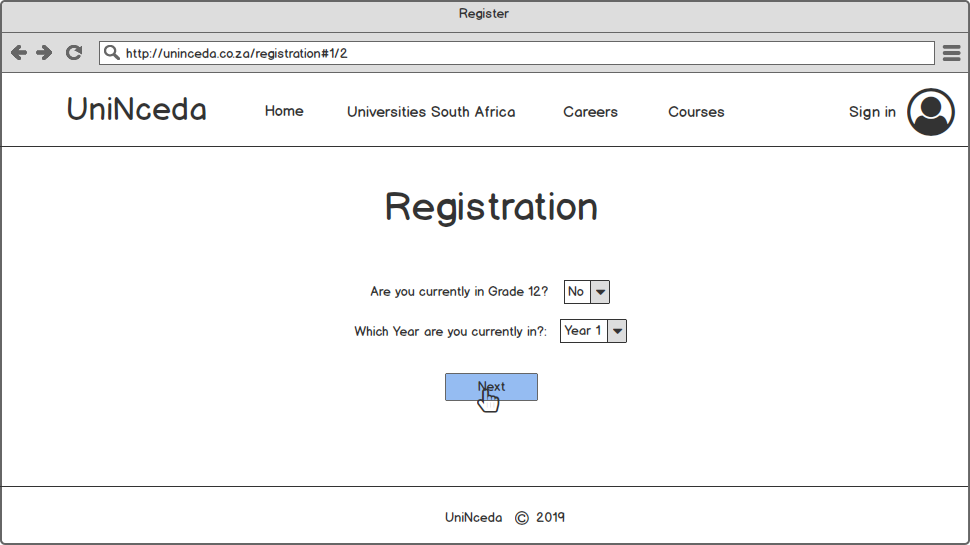
\includegraphics[scale=0.45]{Registration(1)IfNo}
\caption{ In the above mockup the user selected No for the first question and so the second question is enabled. After that the user can click next to proceed.}
\label{Registration(1)IfNo}
\end{figure}

\begin{figure}[H]
\centering
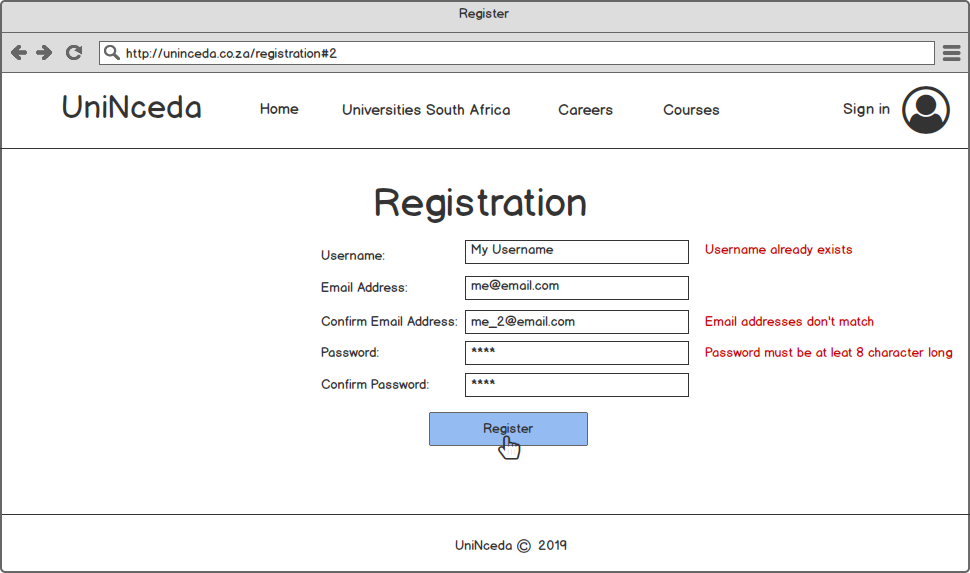
\includegraphics[scale=0.45]{Registration(2)InvalidDetails}
\caption{The user is then presented with a page to enter his/her registration details which are mentioned in \textbf{Section 6:User class}  under \textbf{Registration} and then click Register to proceed.When the user inputs incorrect details into the form the website will display a red coloured error message text next to each textboxes with incorrect input.}
\label{Registration(2)InvalidDetails}

\vspace{1cm}
\setcounter{figure}{1}

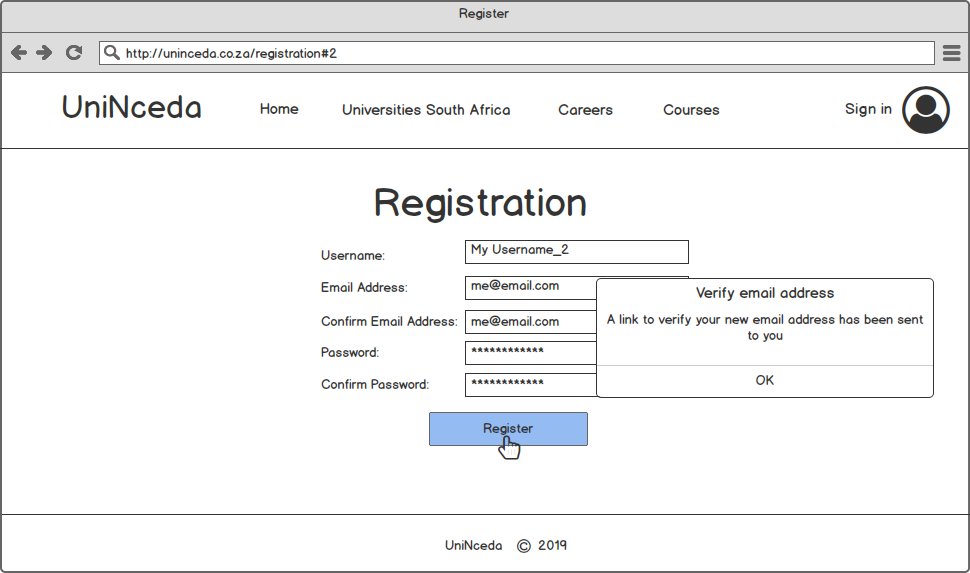
\includegraphics[scale=0.45]{Registration(2)}
\caption{In the above mockup the user inputted the correct details and so an alert box displayed notifying the user to verify the email address through the link sent to it. This is as mentioned in \textbf{Section 6:User Class} under \textbf{Registration}}
\label{Registration(2)}
\end{figure}

\begin{figure}[H]
\centering
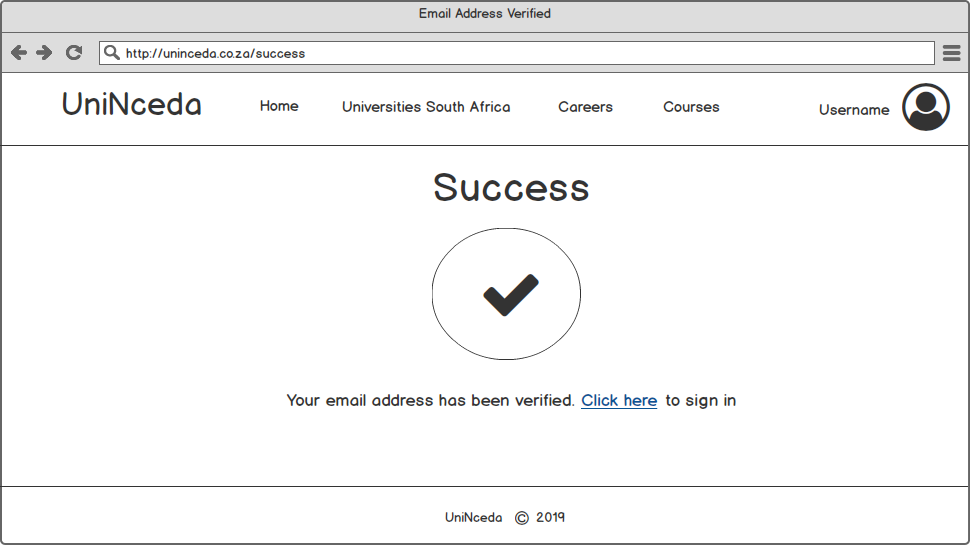
\includegraphics[scale=0.5]{EmailAddressVerified}
\caption{As mentioned in \textbf{Section 6:User class 6} under \textbf{Registration}, the above mockup shows the page that displays when the user has clicked the link to verify his/her email address. The user can then proceed by clicking the link to sign in.}
\label{EmailAddressVerified}
\end{figure}

\FloatBarrier

\subsection{The Login process}

\setcounter{figure}{0}

\begin{figure}[H]
\centering
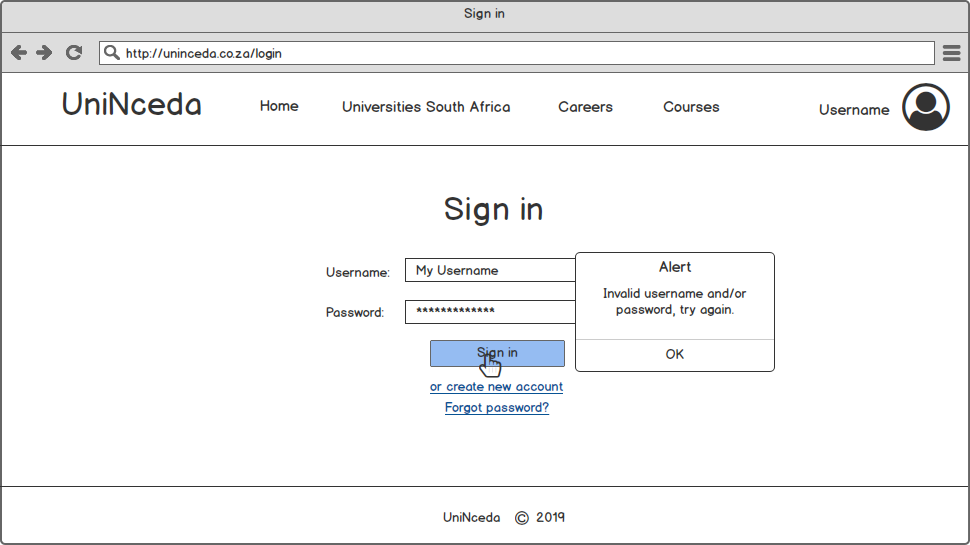
\includegraphics[scale=0.5]{LoginPageInvalidCredentials}
\caption{\small In the above mockup, the user is presented with a page to input login credentials which are his/her username and password and then click sign in to login to his/her account. The user here has inputted invalid login details and so a message box is displayed with a corresponding error message. When the user clicks OK in the alert box, the textboxes for the login credentials are cleared and then the user can make another attempt to login.}
\label{LoginPageInvalidCredentials}

\setcounter{figure}{0}
\vspace{1cm}

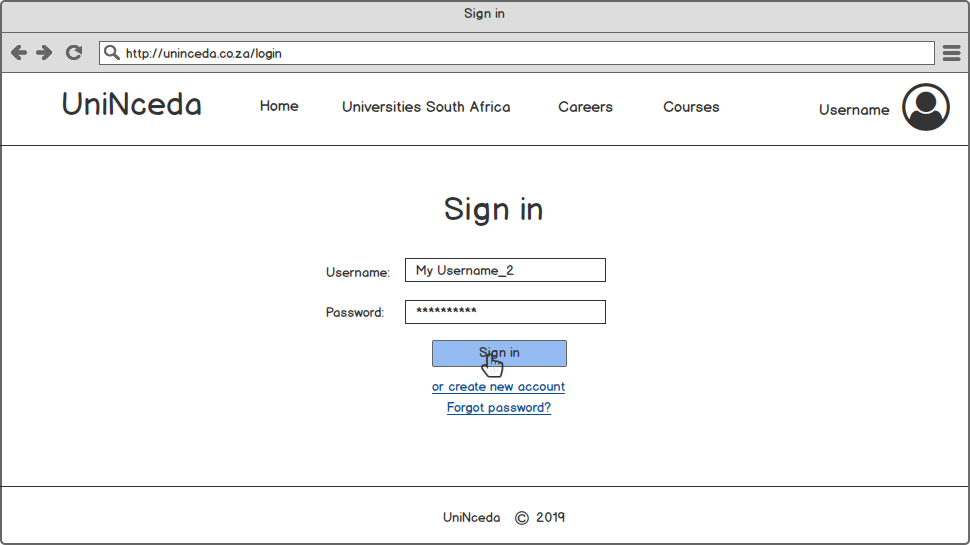
\includegraphics[scale=0.5]{LoginPage}
\caption{\small In the above mockup, the user has now inputted the correct credentials and so when he/she clicks the sign in  button he/she will be given access to his/her account.}
\label{LoginPage}
\end{figure}

\subsection{The Forgot password process}

\setcounter{figure}{0}

\begin{figure}[H]
\centering
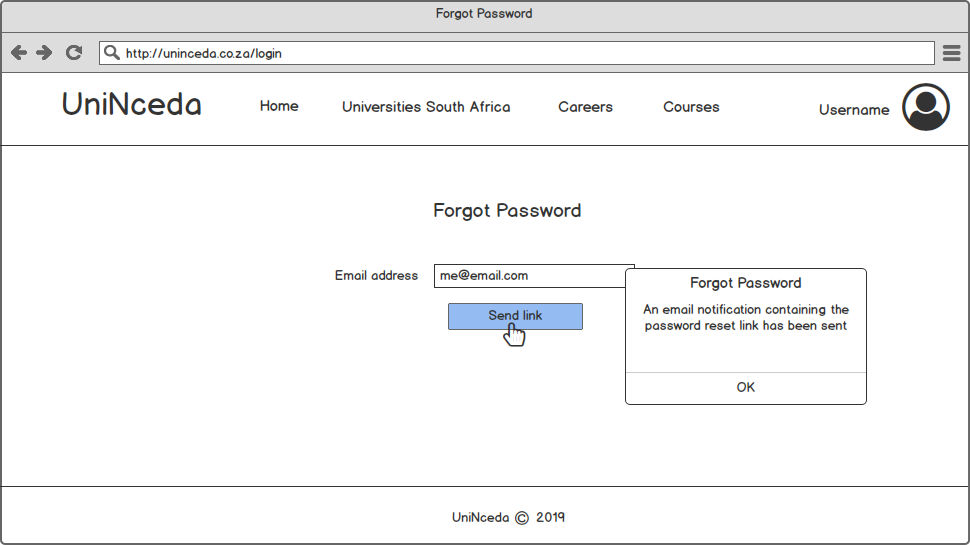
\includegraphics[scale=0.4]{LoginPageForgotPassword}
\caption{\small When the user clicks the forgot password link in the login page he/she is presented with this page. Here the user will input his or her email address as mentioned in \textbf{Section 6:User class} under \textbf{Forgot password} then click the send link button. An alert will display informing the user that an email with the link to reset the password will be sent to the email address.}
\label{LoginPageForgotPassword}

\vspace{1cm}

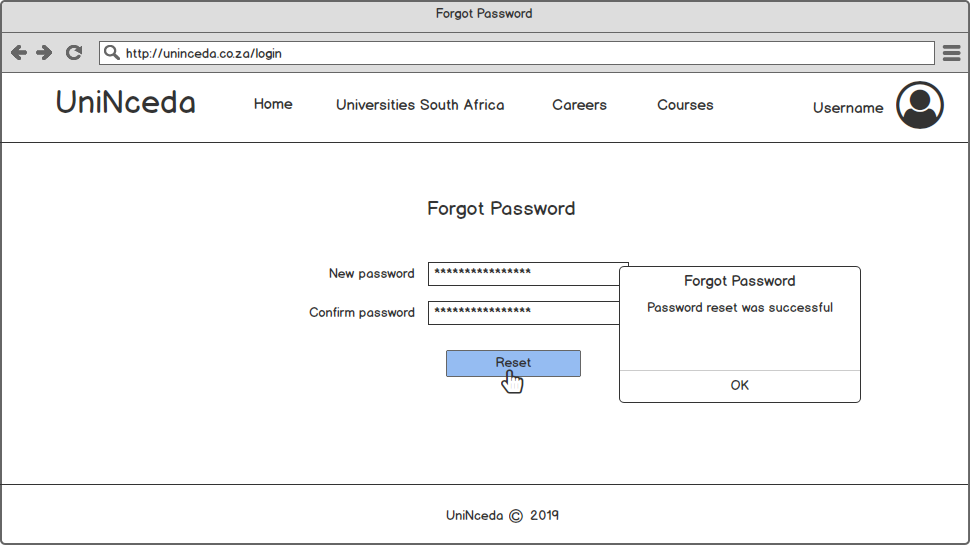
\includegraphics[scale=0.4]{LoginPageForgotPassword(2)}
\caption{\small The above mockup is the page that is presented to the user after he/she has clicked the password reset link sent to his/her email address. Here the user will input the new password and its confirmation then proceed by clicking the reset link. An alert box indicating the success of the password reset process will display. When the user clicks OK he/she will be redirected to the login page.}
\label{LoginPageForgotPassword(2}
\end{figure}

\subsection{Inquiry process (starting from the Home Page)}

\setcounter{figure}{0}

\begin{figure}[H]
\centering
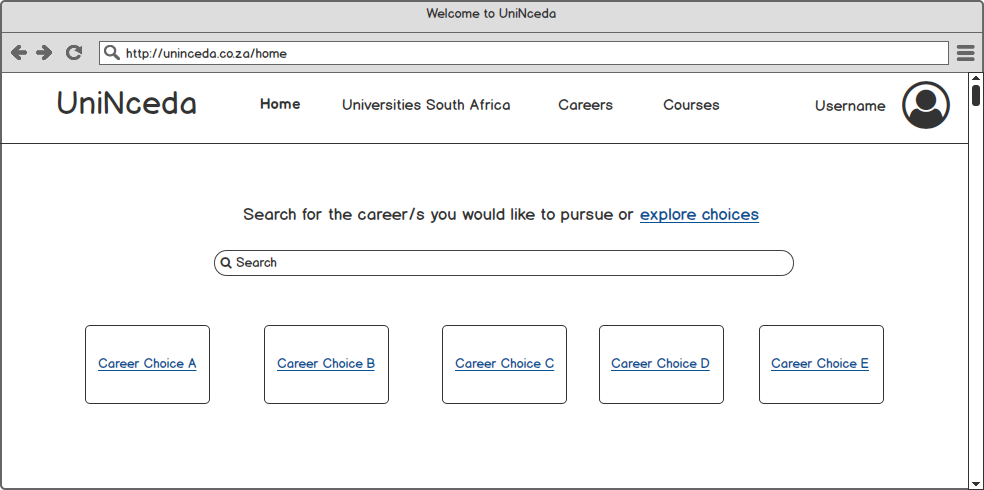
\includegraphics[scale=0.5]{HomePage}
\caption{\small After the login process, the user is presented with the home page. Here the user can search for a career or view the careers page to explore various options. When the user inputs text in the search bar, the results are dynamically shown as seen in the mockup above. After searching, the user can then select any of the career choices displayed in the results, this will redirect the user to the careers page for the career that was selected. This is as mentioned in \textbf{Section 6:User Class} under \textbf{Instant Query Results}}
\label{HomePage}

\vspace{1cm}

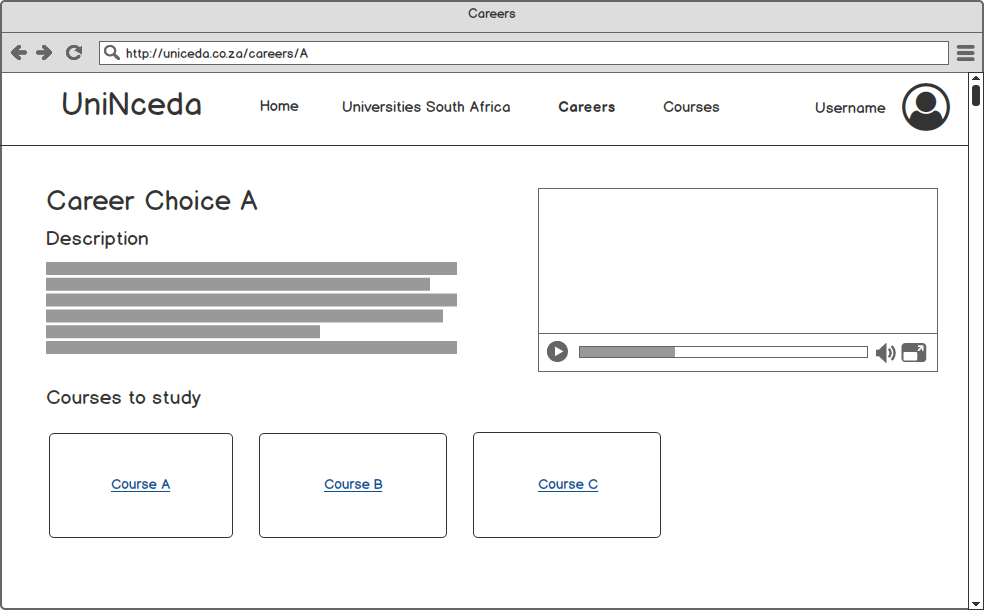
\includegraphics[scale=0.3]{Careers}
\caption{\small The mockup above shows the careers page for a career that the user has previously selected in the home page. Here the user can view more information about the career including descriptions and videos. The user can also view the courses to study to be able pursue that career and not only that but to also navigate through those courses by clicking any of them. This will redirect the user to the courses page.}
\label{Careers}
\end{figure}

\begin{figure}[H]
\centering
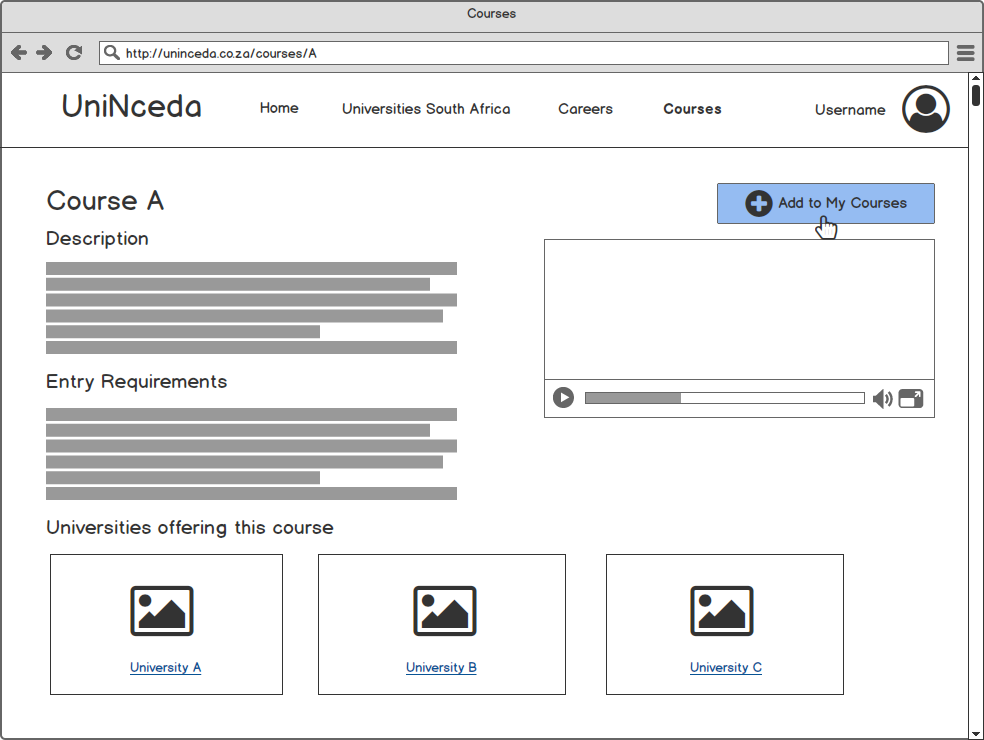
\includegraphics[scale=0.35]{Courses}
\caption{\small \small{The above mockup page is the courses page which shows more information about the course that the user selected from \textbf{Step 2}. The user has the option of adding the course to his/her profile by clicking the 'Add to My Courses' button. The user can view and select any of the universities that are offering the course, this will redirect the user to the 'Universities South Africa' page for the university offering the course.}}
\label{Courses}

\vspace{1cm}

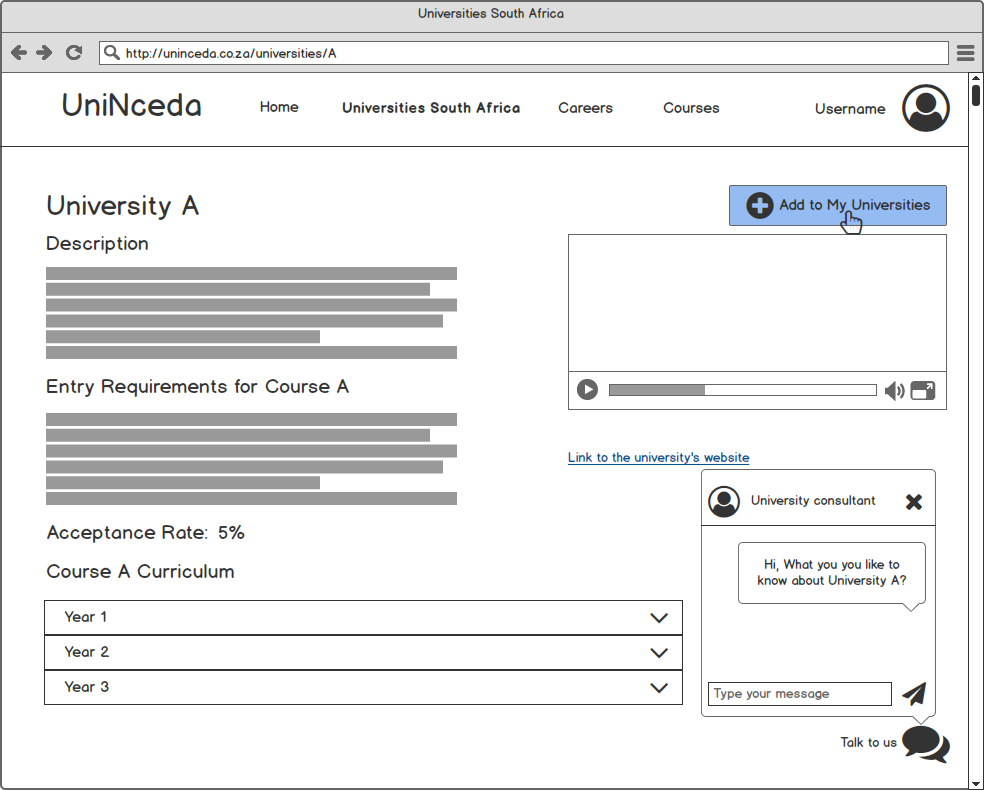
\includegraphics[scale=0.35]{UniversitiesPage1}
\caption{\small \small{After the user has selected the university from \textbf{Step 3}, he/she will be redirected to this page to view more information about the university (description, entry requirements, acceptance rate etc.}. The user can also view the curriculum of the university for the course  the user has selected and not only that but also chat to the university's consultants for that course through the interactive chatbox. The user has the option to add the university to his/her profile through the 'Add to My Universities' button.}
\label{UniversitiesPage1}
\end{figure}

\begin{figure}[H]
\centering
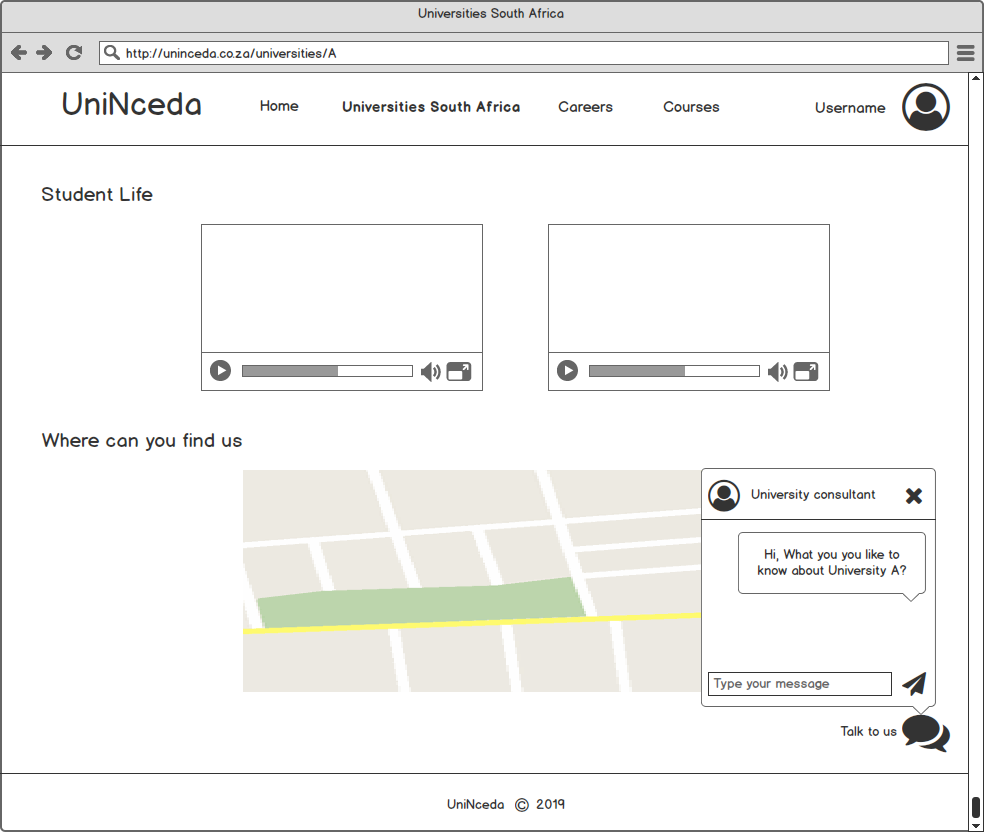
\includegraphics[scale=0.5]{UniversitiesPage2}
\caption{\small \small{The above mockup page is the content displayed after the user has scrolled down to the end of the page. It consists of even more information about the university (student life and location). The chatbox remains active on scroll so that the user can continue chatting to the university's officials. This is as mention in \textbf{Section 6:User Class} under \textbf{Real-Time Communication With University Officials}.}}
\label{UniversitiesPage2}
\end{figure}

\newpage

\subsection{Page Navigation}
\renewcommand{\figurename}{Figure}
\setcounter{figure}{0}
The following mockups show the main pages of the website that the user would navigate to in any order or flow.

\begin{figure}[H]
\centering
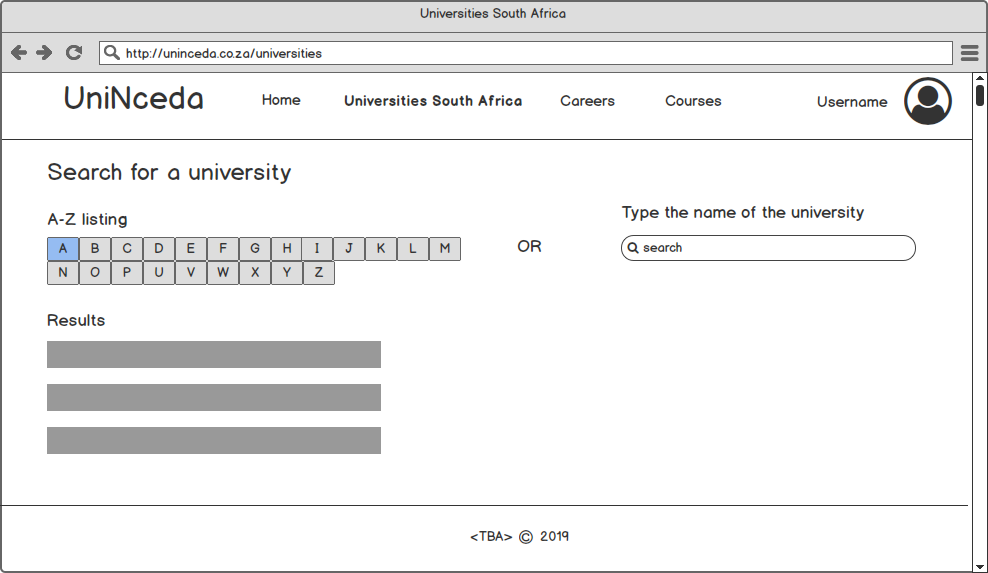
\includegraphics[scale=0.4]{UniversitiesSouthAfrica}
\caption{The above mockup is the 'Universities South Africa' page, here the user can search for any university by either selecting from the A-Z listing or by inputting text into the search bar. The results of the search will then display below.}
\label{UniversitiesSouthAfrica}

\vspace{1cm}

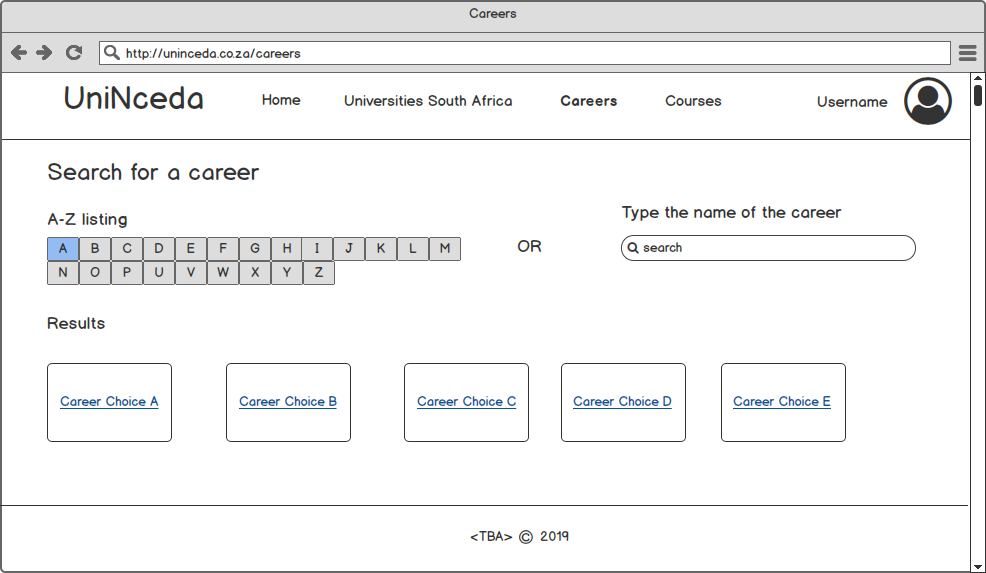
\includegraphics[scale=0.4]{CareersPage}
\caption{The above mockup is the 'Careers' page, as in \textbf{Figure 1} the user here can search for any career by either selecting from the A-Z listing or by inputting text into the search bar. The results of the search will then display below.}
\label{CareersPage}
\end{figure}

\begin{figure}[H]
\centering
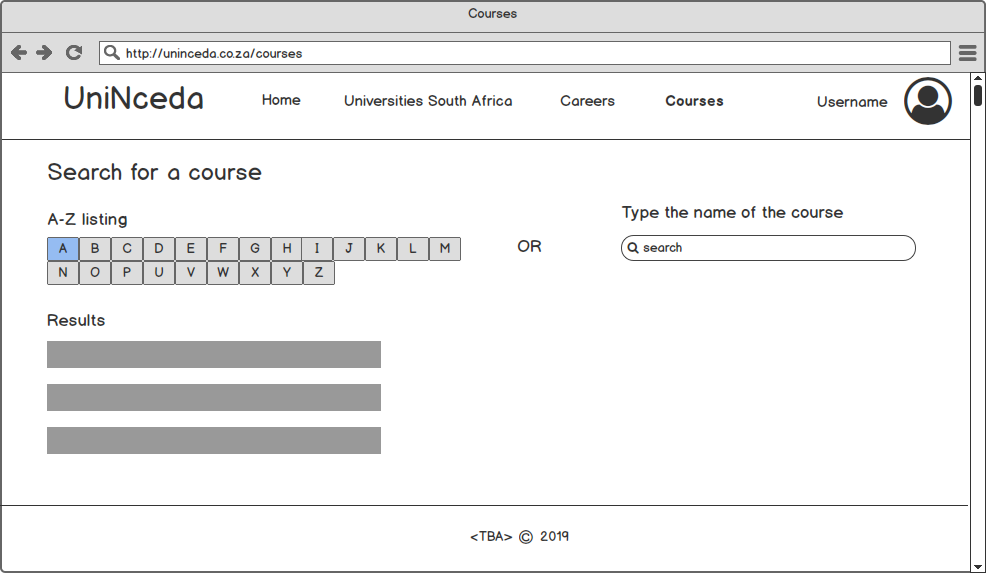
\includegraphics[scale=0.3]{CoursesPage}
\caption{The above mockup is the 'Courses' page, as in \textbf{Figure 2} the user here  can search for any course by either selecting from the A-Z listing or by inputting text into the search bar. The results of the search will then display below.}
\label{CoursesPage}

\vspace{1cm}

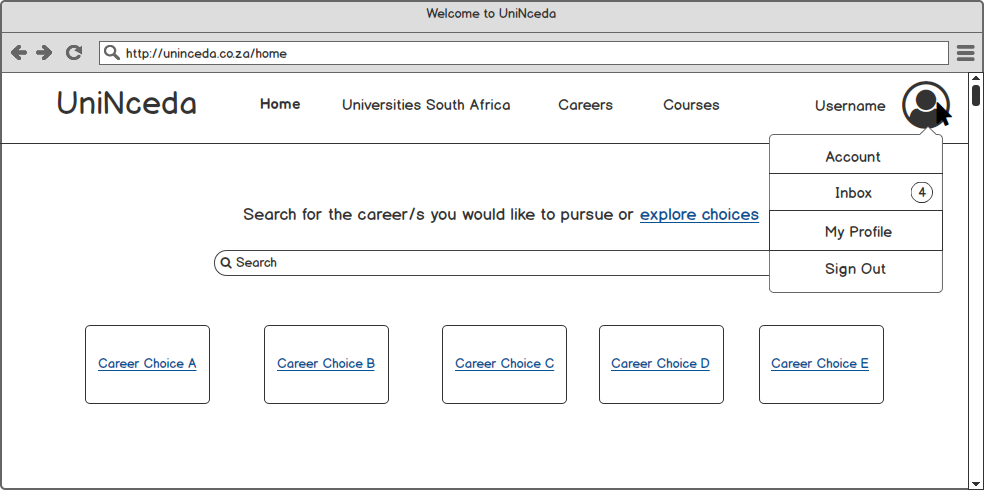
\includegraphics[scale=0.4]{HomePageNav}
\captionsetup{singlelinecheck=off}
\caption[foo bar]{The above mockup shows the dropdown menu that displays when the user clicks on the 'user icon' on the navigation bar. The dropdown menu consists of four links.

\begin{enumerate}
\item \textbf{Account link} - Clicking this link will redirect the user to the 'Account' page. This is where the user can view or edit his/her account information.
\item \textbf{Inbox link} - Clicking this link will redirect the user to the 'Inbox' page. This is where the user can view his/her latest notifications.
\item \textbf{My Profile link} - Clicking this link will redirect the user to the 'My Profile' page. This is where the user can build his/her profile by inputting information into the various forms.
\item \textbf{Sign Out link} - Clicking this link will log the user out of his/her account and redirect the user to the home page.
\end{enumerate}

 }
\label{HomePageNav}
\end{figure}

\newpage
\subsection{Viewing and Editing Account Information}
The subsequent mockups are related to the functional requirements in \textbf{Section 6:User Class} under \textbf{Viewing and Editing Account Information}.
\setcounter{figure}{0}

\begin{figure}[H]
\centering
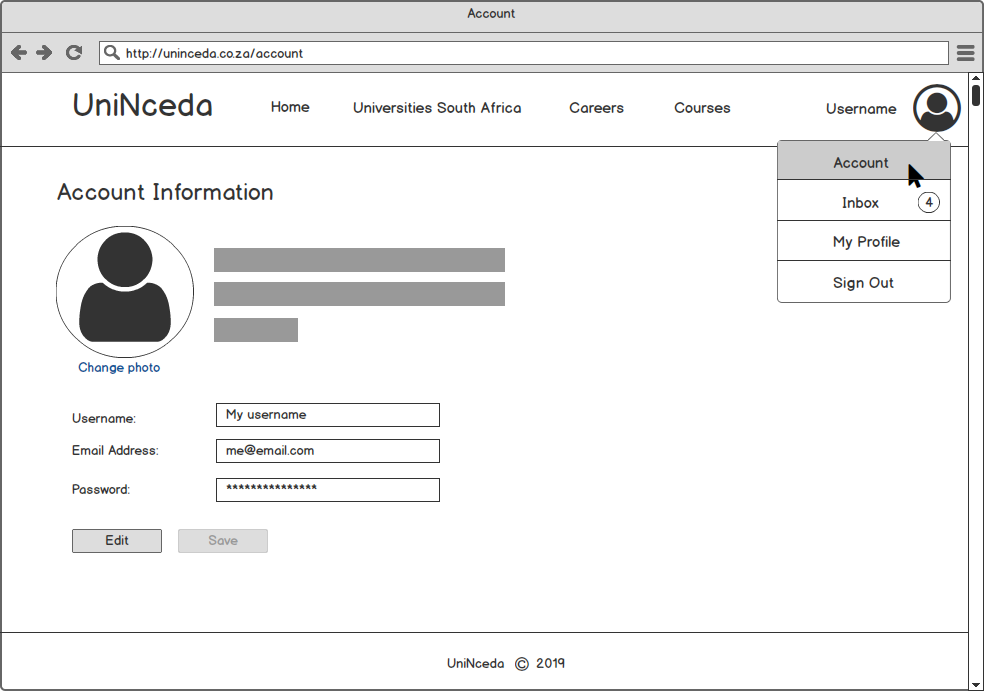
\includegraphics[scale=0.35]{Account}
\caption{The above mockup is the 'Account' page. Here the user is able to view his/her account information.}
\label{Account}

\vspace{1cm}

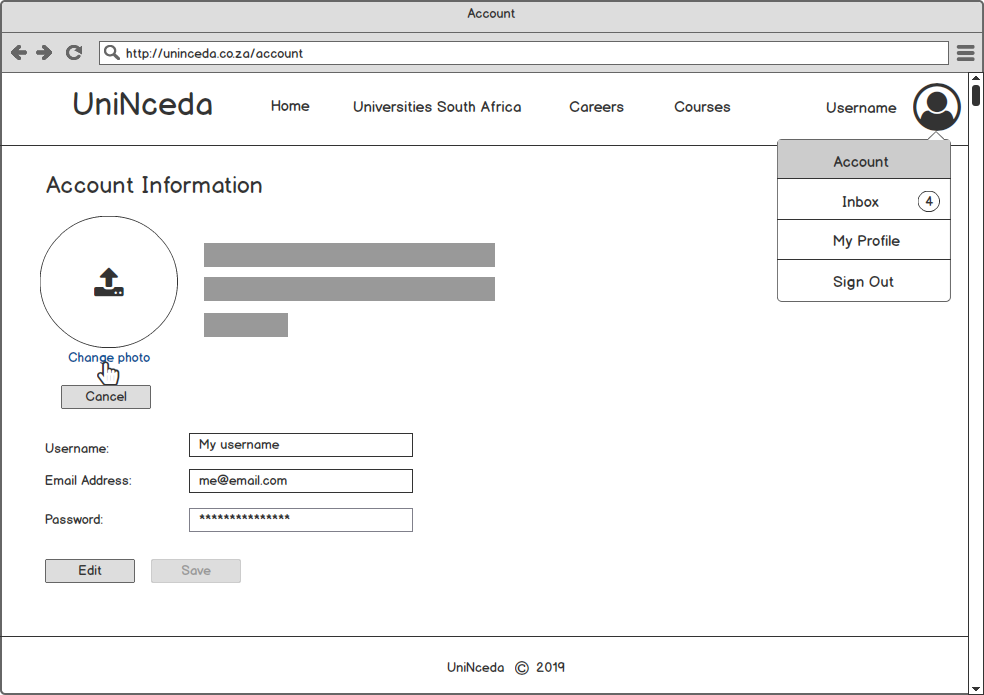
\includegraphics[scale=0.35]{AccountPhotoChange}
\caption{The above mockup is the 'Account' page. Here the user has clicked the 'Change photo' link and so the website responded accordingly by displaying the upload button control that will enable the user to upload a new image. If the user decides to terminate this process and revert to the old image he/she can click the 'Cancel' button.}
\label{AccountPhotoChange}
\end{figure}

\renewcommand{\figurename}{Step}
\setcounter{figure}{0}

\begin{figure}[H]
\centering
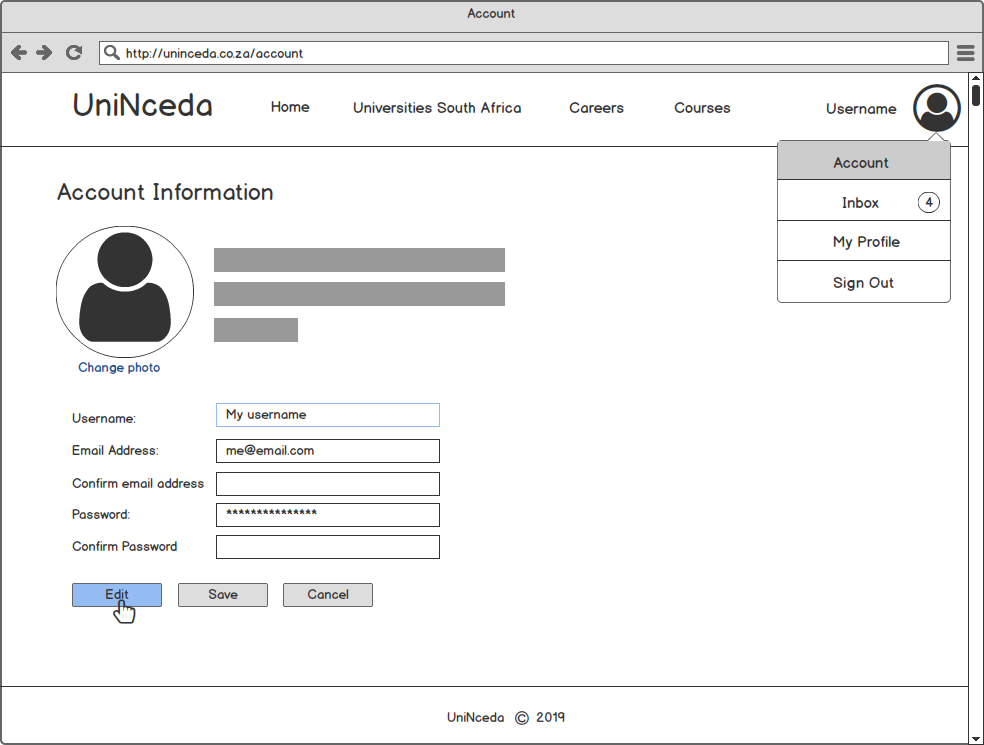
\includegraphics[scale=0.4]{AccountChangingDetails}
\caption{The above mockup is the 'Account' page. Here the user has clicked the 'Edit' button and so the 'Confirm Email Address' and the 'Confirm Password' field appeared enabling the user to change the existing username, email address and password.}
\label{AccountChangingDetails}

\vspace{1cm}

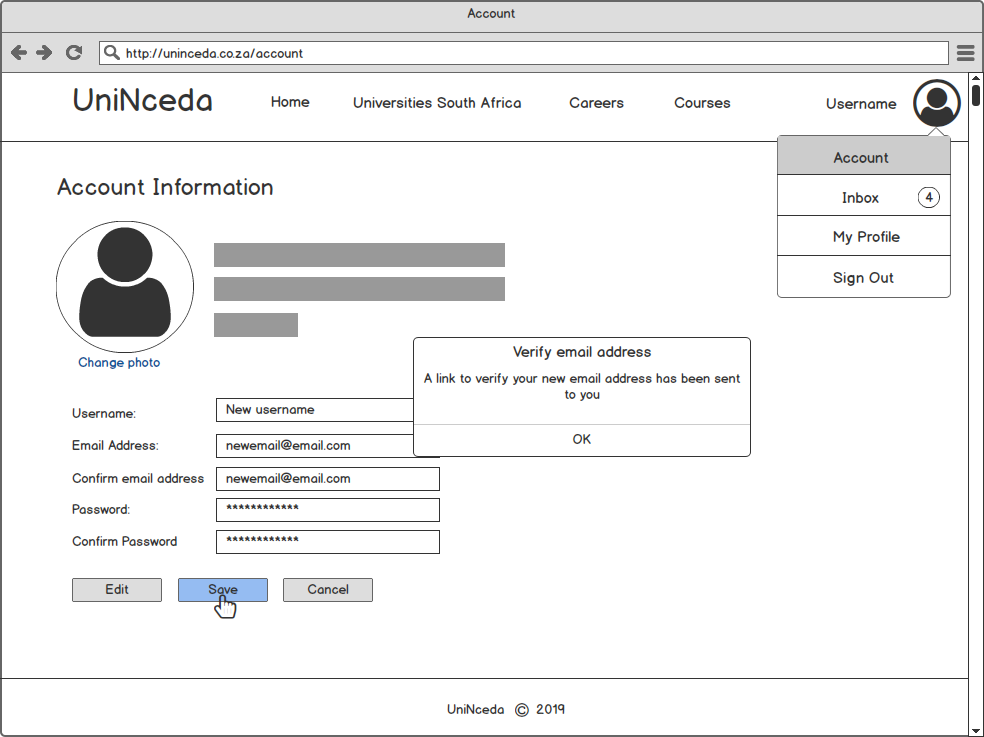
\includegraphics[scale=0.4]{AccountChangingDetailsSave}
\caption{The above mockup is the 'Account' page. Here the user has clicked the 'Save' button and so the details are then saved into the user's account. An alert box that notifies the user to verify a new email address is displayed accordingly if the user changed his/her old email address.}
\label{AccountChangingDetailsSave}
\end{figure}

\subsection{Checking Inbox}

\renewcommand{\figurename}{Figure}
\setcounter{figure}{0}

\begin{figure}[H]
\centering
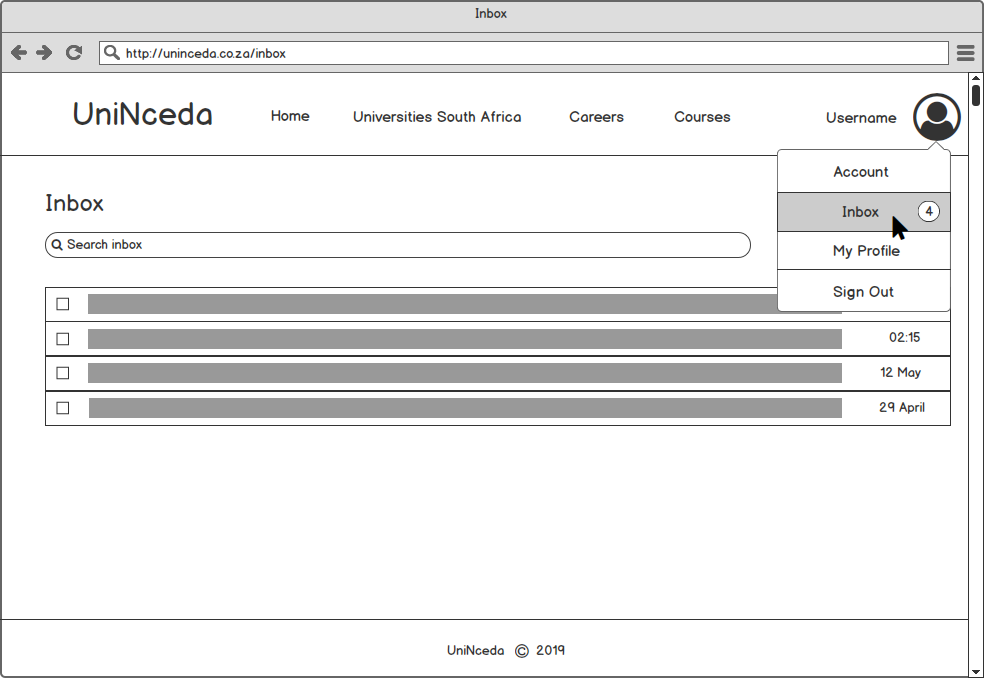
\includegraphics[scale=0.5]{Inbox}
\caption{The mockup above is the 'Inbox' page. Here the user is able to view the latest notifications sent to him or her from the universities, this includes notifications about the application deadlines, acceptance etc. This is as mentioned in \textbf{Section 6:User Class} under \textbf{Receiving Notifications}}
\label{Inbox}
\end{figure}

\newpage
\subsection{Profile Creation}
The subsequent sections are for the mockups in the 'My Profile' page they are related to the functional requirements in \textbf{Section 6:User Class} under \textbf{Building a Profile}. On the left of these mockups is a navigation bar that enables the user to navigate through the various pages.
\subsubsection{Filling in Application Information}
The subsequent mockups are for the 'Application Information' section of the 'My Profile' page. The user can access this section by clicking the corresponding link on the navigation bar, this will display the various pages contained within the section in a dropdown list below. Each page contains a form that has three buttons, the 'Save' button which enables the user to save his/her current progress, the 'Clear' button which clears all the text fields and resets all the controls in the form, and lastly the 'Submit' button which stores the user's error free data into a secure database and redirects the user to the next page.
\renewcommand{\figurename}{Step}
\setcounter{figure}{0}

\begin{figure}[H]
\centering
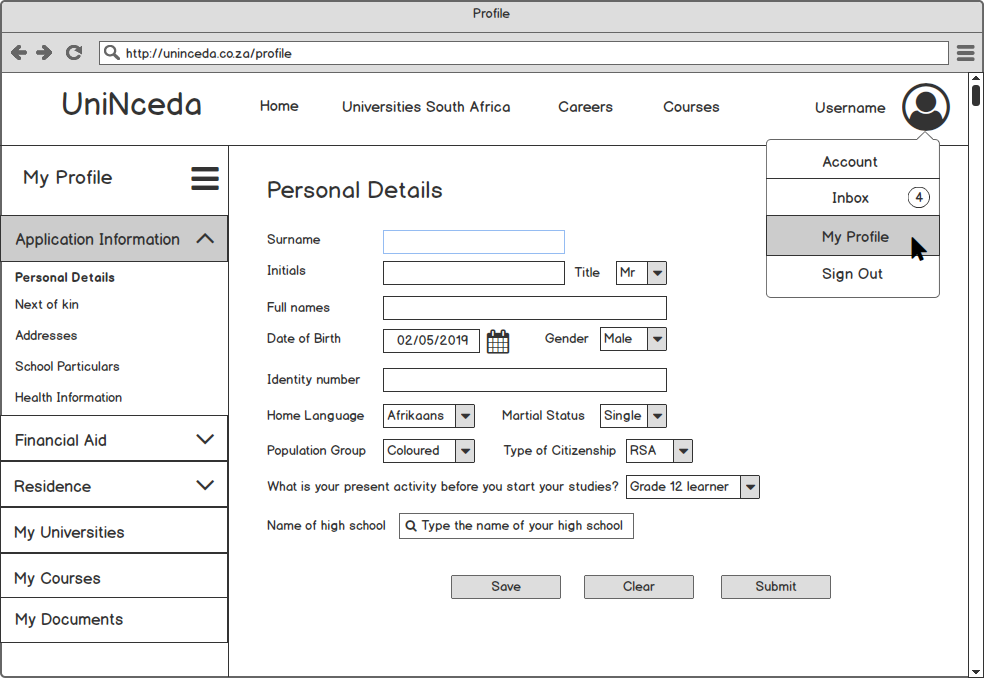
\includegraphics[scale=0.4]{ProfileAppInfoPersonalDetailsOpt(1)}
\caption{The above mockup is the 'Personal Details' page. Here the user is presented with a form to fill in his/her personal details (surname, name, date of birth etc.). After filling in the form successfully the user can click the 'Submit' button which will validate the data inputted into the form and if it is correct, it will redirect the user to the 'Next of kin' page. This page is presented to a current high school student.}
\label{ProfileAppInfoPersonalDetailsOpt(1)}
\end{figure}

\setcounter{figure}{0}

\begin{figure}[H]
\centering
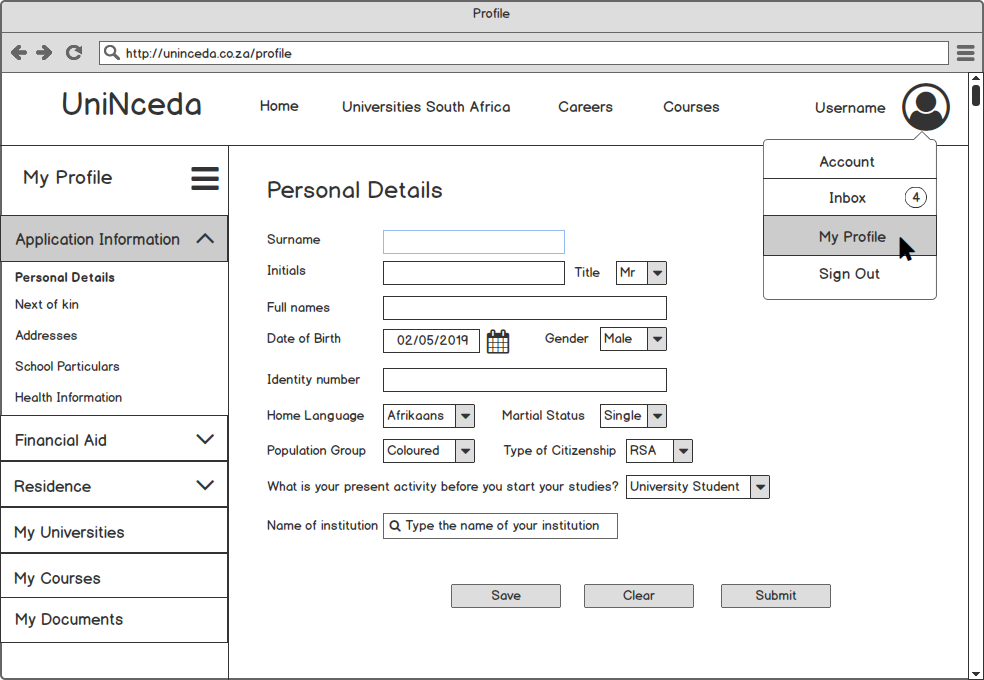
\includegraphics[scale=0.4]{ProfileAppInfoPersonalDetailsOpt(2)}
\caption{The above is the same as the one in \textbf{Step 1}. This page is presented to a current university student.}
\label{ProfileAppInfoPersonalDetailsOpt(2)}
\end{figure}

\begin{figure}[H]
\centering
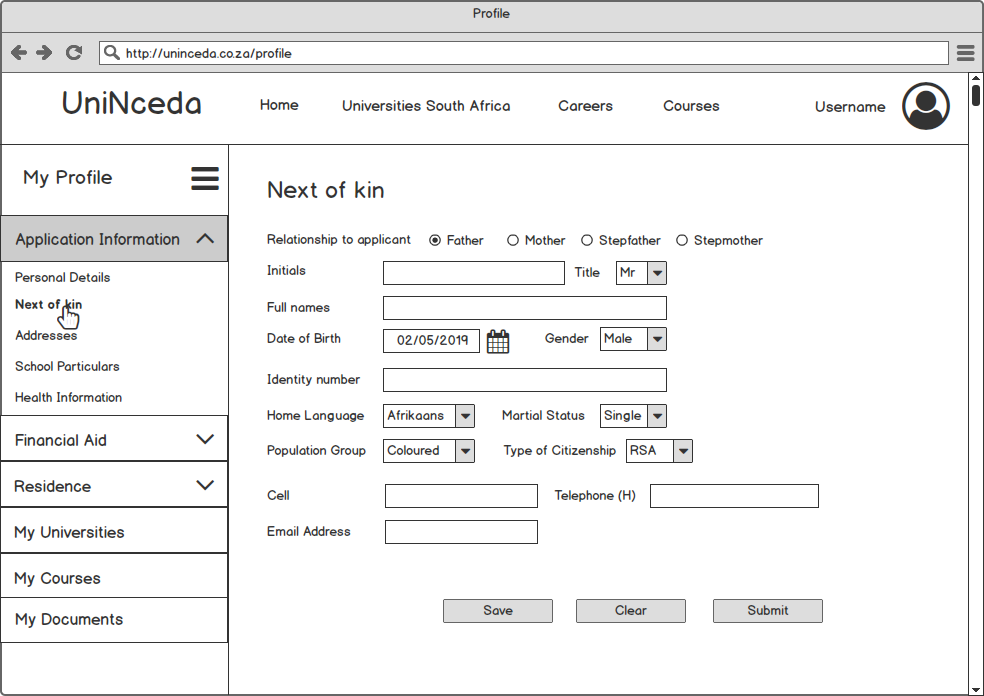
\includegraphics[scale=0.4]{ProfileAppInfoNextOfKin}
\caption{The user is presented with a form to be filled in by his/her next of kin. When the user clicks the 'Submit' button, the information is validated and if correct the user will be redirected to the 'Addresses' page.m This form is only presented to users under the age of 18, otherwise the user will be redirected to the 'Addresses' page.}
\label{ProfileAppInfoNextOfKin)}
\end{figure}

\begin{figure}[H]
\centering
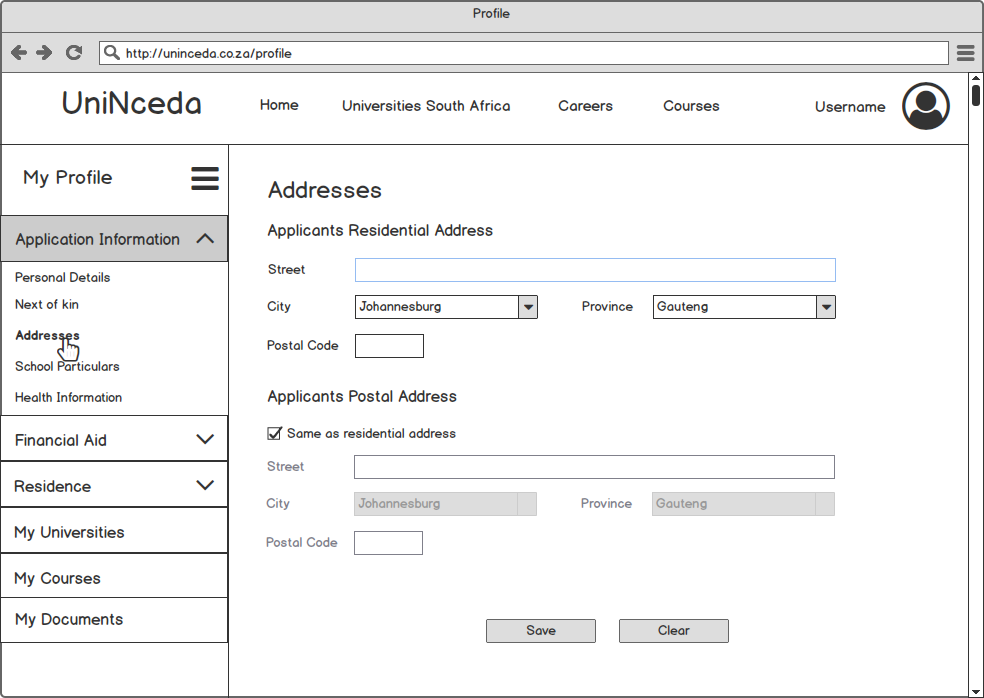
\includegraphics[scale=0.35]{ProfileAppInfoAddresses}
\caption{The user is presented with a form to input address information (residential address and postal address). When the user checks the 'Same as residential address' checkbox the input fields it below are disabled. After filling in the information successfully, the user can scroll down to proceed.}
\label{ProfileAppInfoAddresses}

\vspace{1cm}

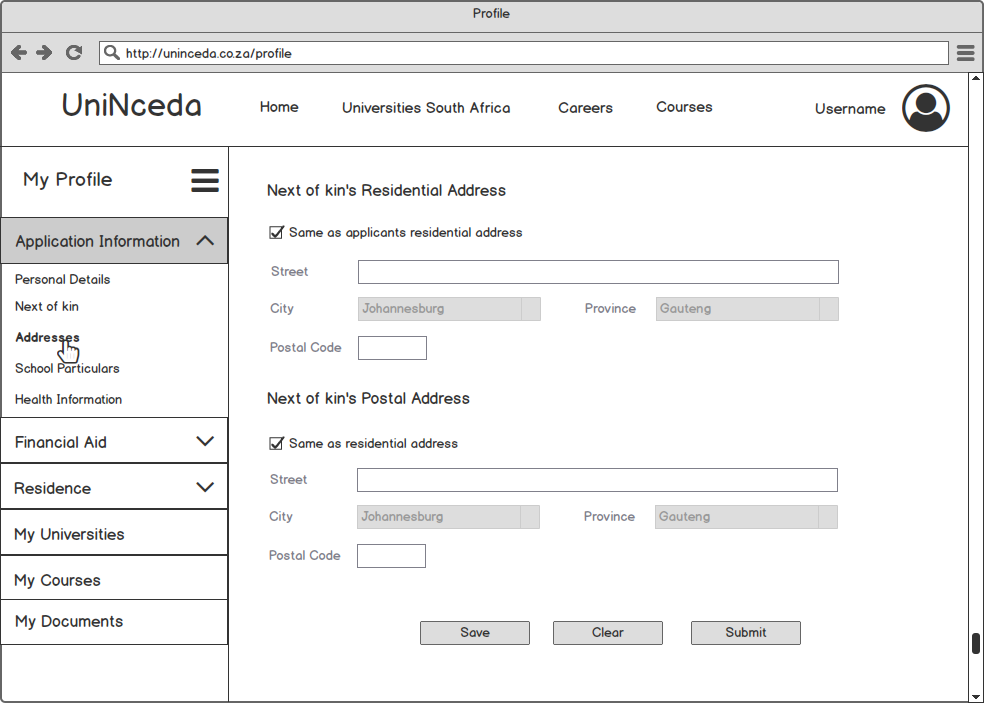
\includegraphics[scale=0.35]{ProfileAppInfoAddressesPage2}
\caption{This part of the page appears when the user scrolls down to end to the page. Here the user is presented with a form to input the next of kin's address information.When the checks the 'Same as applicant's residential address' checkbox the input fields below it are disabled, the same applies to the 'Same as residential address' checkbox. After filling in the required information, the user can click the 'Submit' button which will validate the information inputted into the form and redirect the user to the 'School Particulars' page. }
\label{ProfileAppInfoAddressesPage2)}
\end{figure}

\begin{figure}[H]
\centering
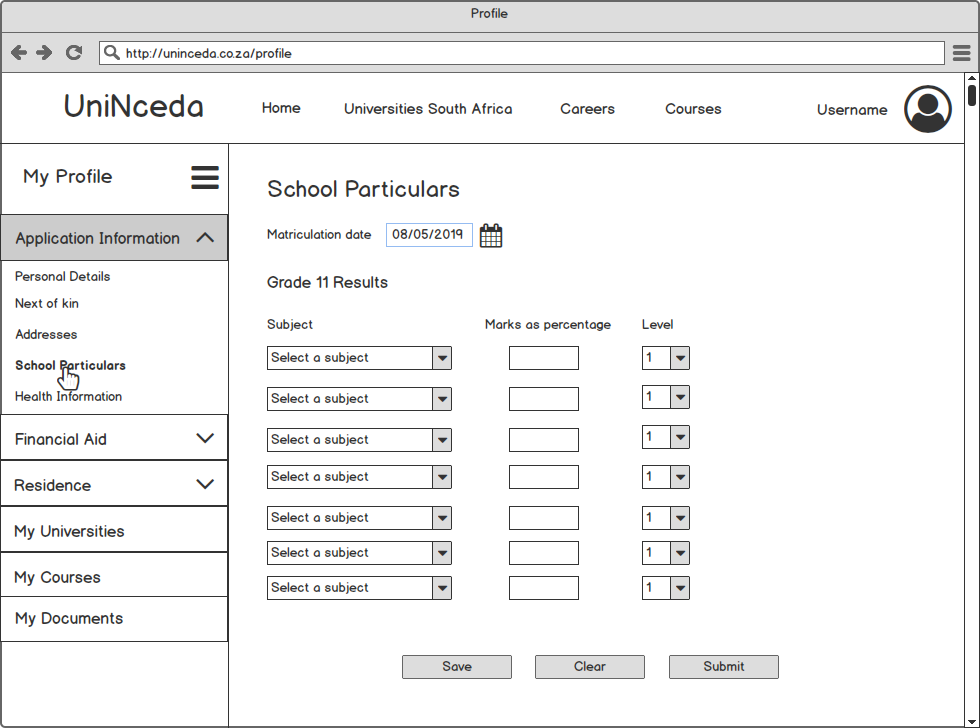
\includegraphics[scale=0.4]{ProfileAppInfoSchoolParticulars}
\caption{The user is presented with this form to  input his/her matriculation date and Grade 11 results. The user does this by selecting a subject ,typing in the obtained mark as a percentage and selecting the subject level. When the user clicks the 'Submit' button the form is validated and the user is redirected to the 'Health Information' page.}
\label{ProfileAppInfoSchoolParticulars}

\vspace{1cm}

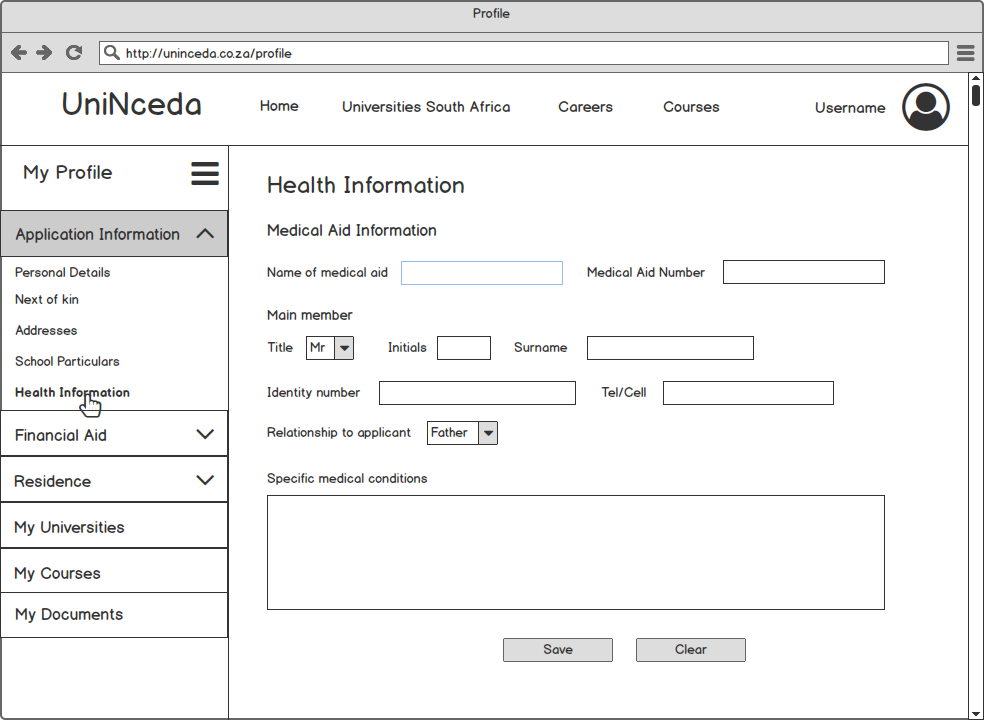
\includegraphics[scale=0.4]{ProfileAppInfoHealthInformation}
\caption{The user is presented with this form to input his/her medical aid information (if available). The user can then scroll down to finish filling in the rest of the form. This form is optional so the user can choose to skip it.}
\label{ProfileAppInfoHealthInformation}


\end{figure}

\begin{figure}[H]
\centering

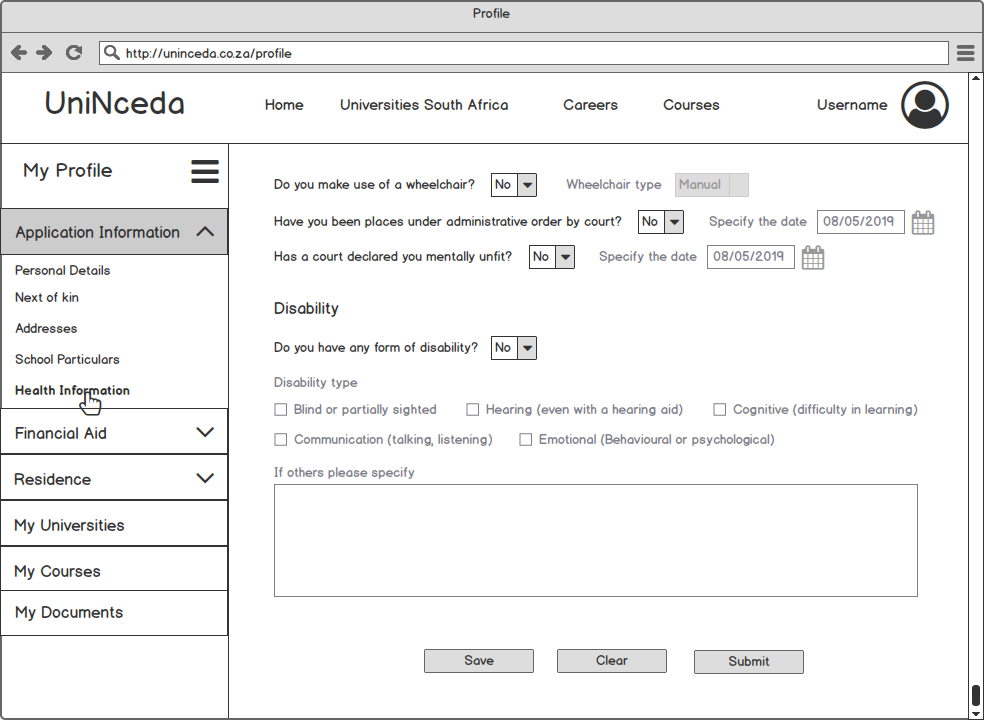
\includegraphics[scale=0.5]{ProfileAppInfoHealthInformationPage2}
\caption{When the user scrolls down to end of the page he/she is presented with this part of the form to input information about his/her disability. When the user selects 'No' for the question 'Do you have any form of disability?', the input fields below it are then disabled. The user can click the 'Submit' button when finished with filling in the form, this will then validate the form. }
\label{ProfileAppInfoHealthInformationPage2}


\end{figure}

\newpage
\subsubsection{Viewing Financial Aid Information}

\setcounter{figure}{0}

\begin{figure}[H]
\centering
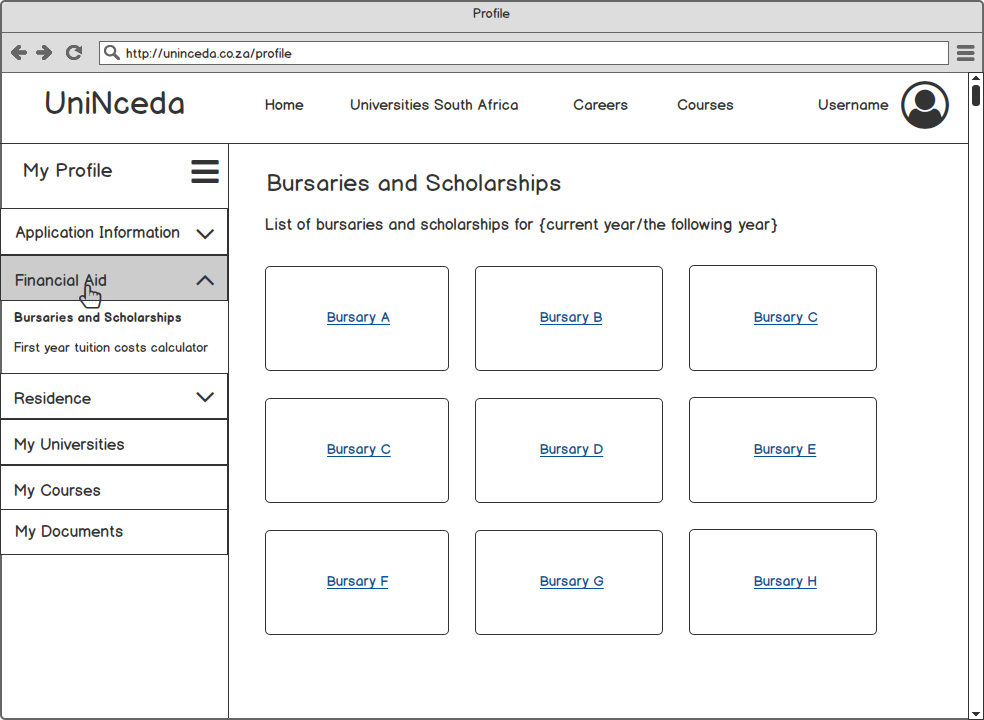
\includegraphics[scale=0.35]{ProfileFinancialAidBursaries}
\caption{In the bove mockup, the user is presented with the 'Bursaries and Scholarships' page that lists the bursaries and scholarships available for that current year. The user can scroll down to view more information.}
\label{ProfileFinancialAidBursaries}

\vspace{1cm}

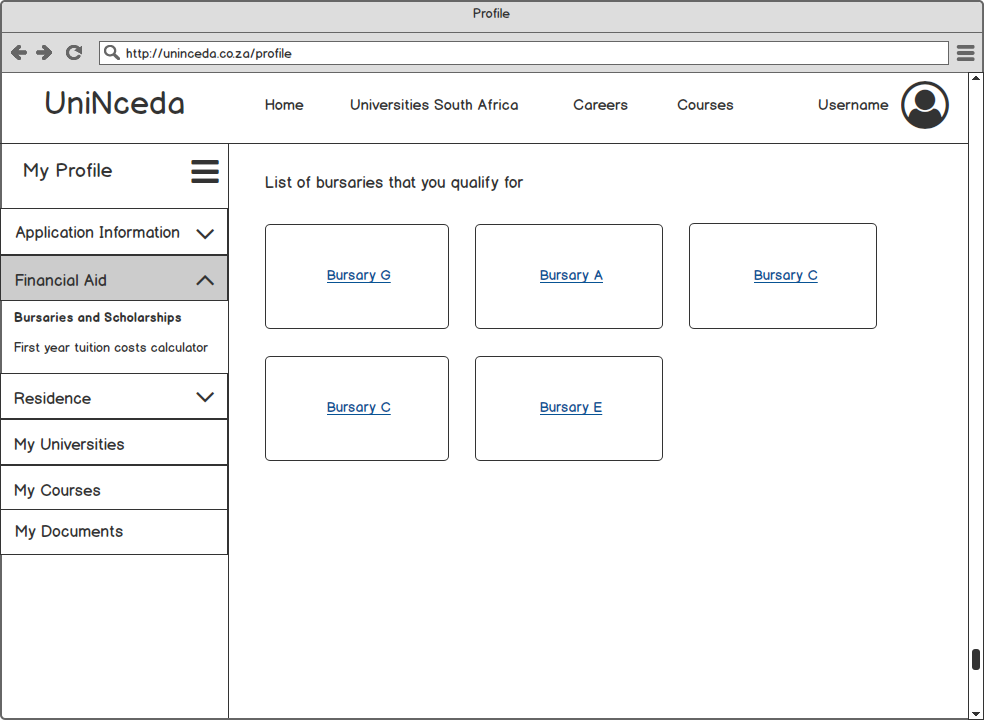
\includegraphics[scale=0.35]{ProfileFinancialAidBursariesPage2}
\caption{This page appears when the user scrolls to end of the page. Here the user is presented with a list of bursaries he/she qualifies for based of his/her final results.}
\label{ProfileFinancialAidBursariesPage2}

\end{figure}

\setcounter{figure}{1}

\begin{figure}[H]
\centering

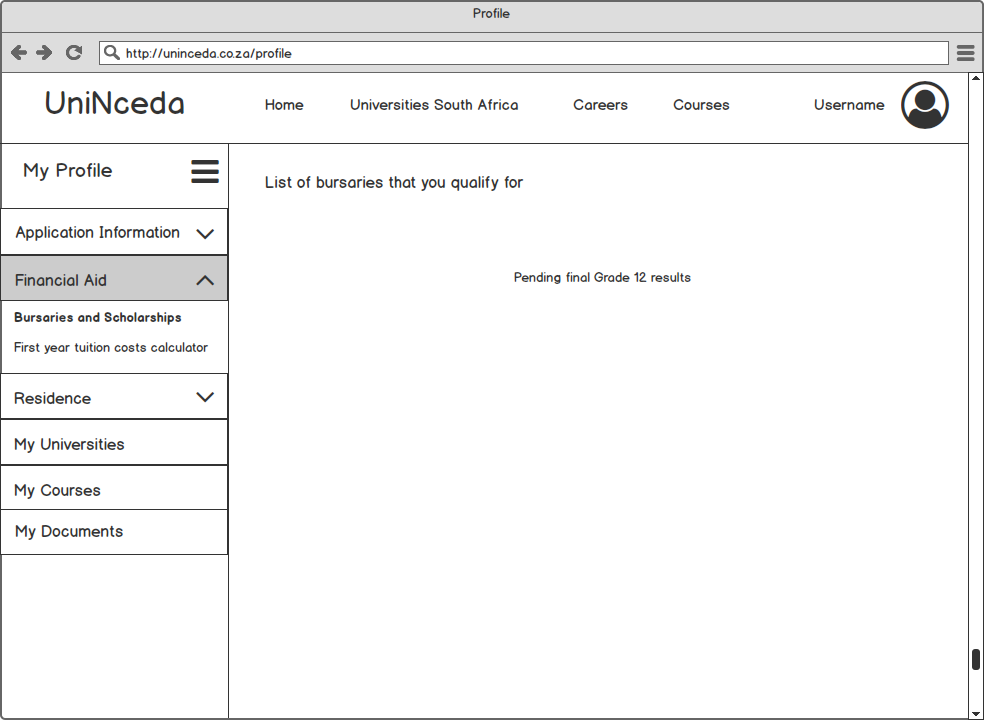
\includegraphics[scale=0.4]{ProfileFinancialAidBursariesPage2NoResults}
\caption{This page appears when the user scrolls to end of the page. Here the message 'Pending final Grade 12 results' has appeared because the user hasn't yet uploaded his/her final results.}
\label{ProfileFinancialAidBursariesPage2NoResults}

\vspace{1cm}

\renewcommand{\figurename}{Figure}
\setcounter{figure}{0}

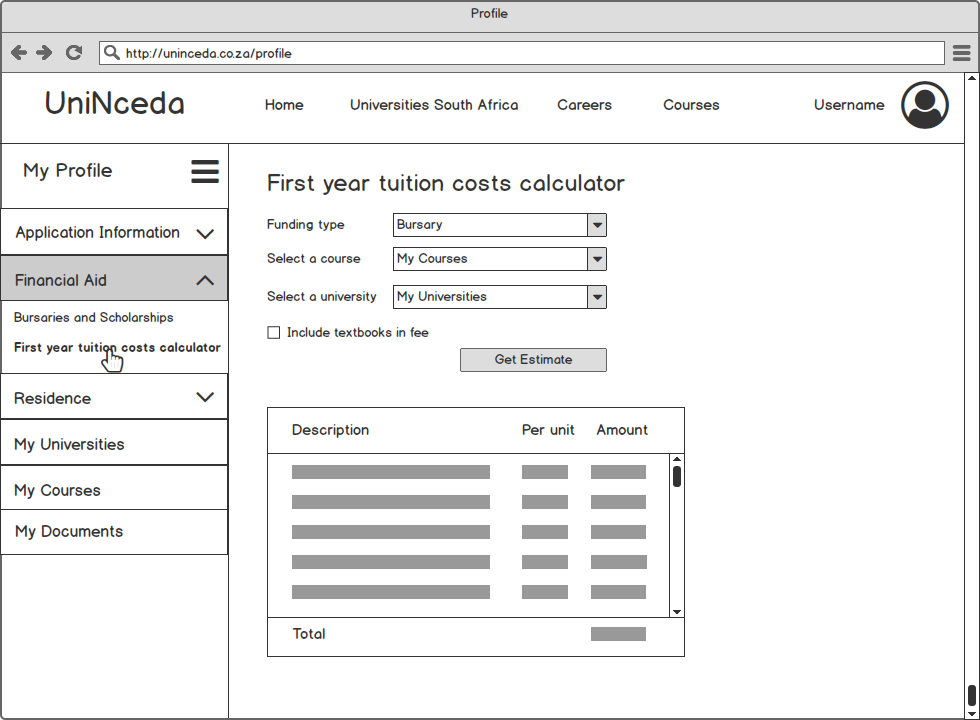
\includegraphics[scale=0.4]{ProfileFinancialAidFeesEstimator}
\caption{Here the user is presented with a form to calculate his/her first year tuition costs based his/her selections. After the user makes the selections he/she can click the 'Get Estimate' button which will show the price estimates in the container below.}
\label{ProfileFinancialAidFeesEstimator}

\end{figure}

\subsubsection{Viewing and editing My Residences}

\setcounter{figure}{0}

\begin{figure}[H]
\centering
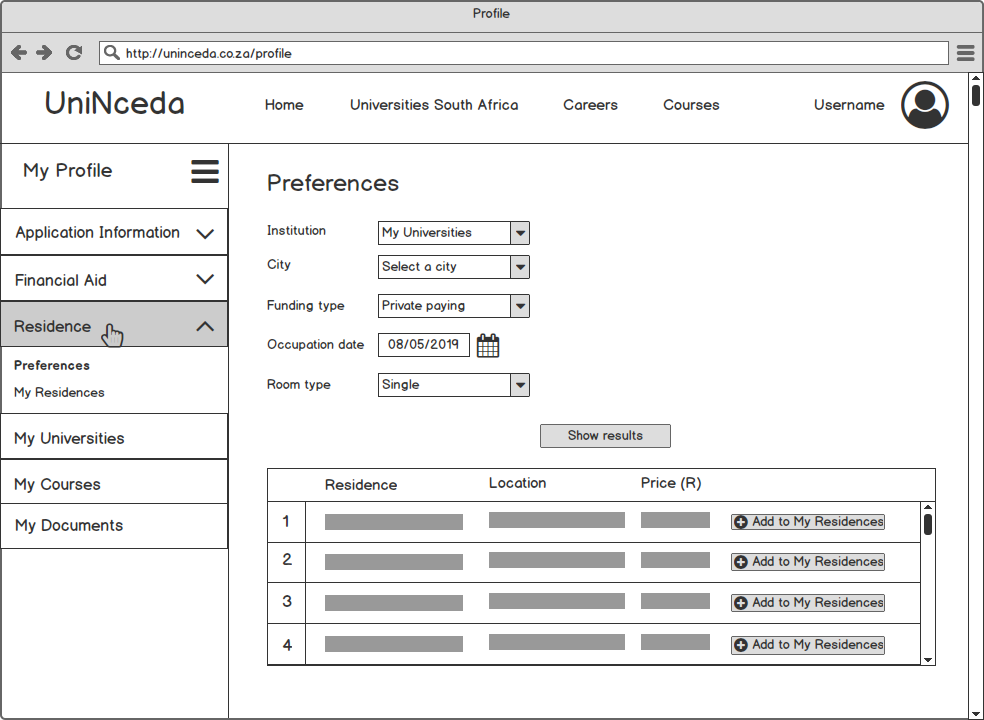
\includegraphics[scale=0.35]{ProfileResidencePreferences}
\caption{The user is presented with a form to create preferences of the residences that he/she wants. After making the selections, the user must click the 'Show Results' button which will show a list of residences that fit the user's preferences in the container below. The user is also able to add any of these residences to 'My Residences' by clicking the 'Add to My Residences' button next to the corresponding residence.}
\label{ProfileResidencePreferences}

\vspace{1cm}

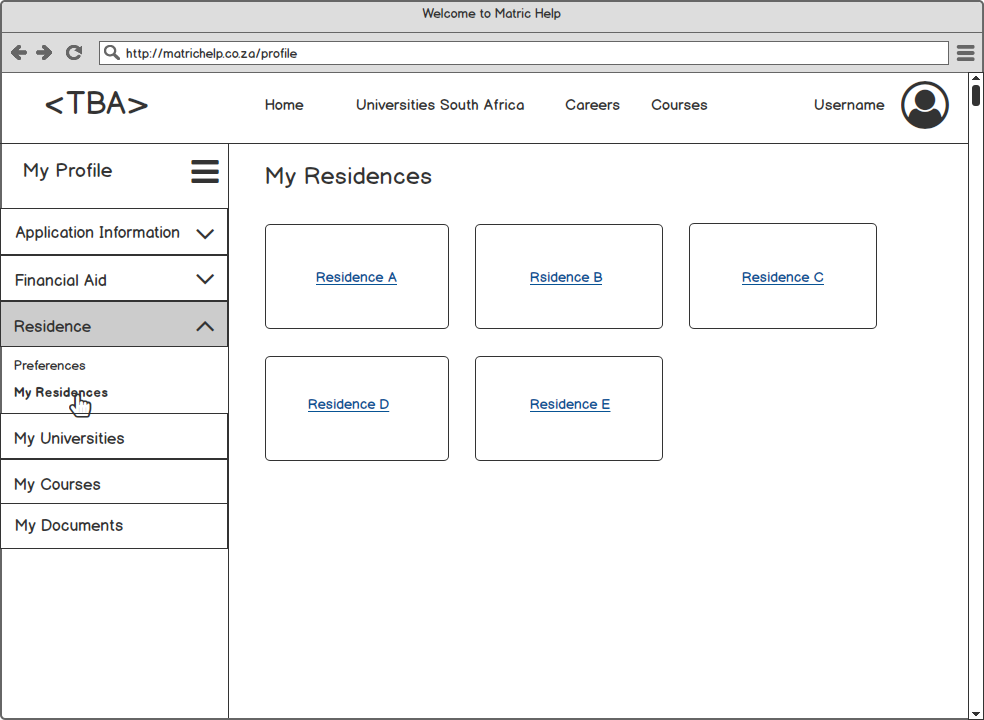
\includegraphics[scale=0.35]{ProfileResidenceResidences}
\caption{Here the user is presented with a list of residences that he/she added. The user is able to click the link at any residence, which will redirect the user to the website for that residence on a new tab.}
\label{ProfileResidenceResidences}


\end{figure}

\renewcommand{\figurename}{Figure}
\setcounter{figure}{0}

\begin{figure}[H]
\centering
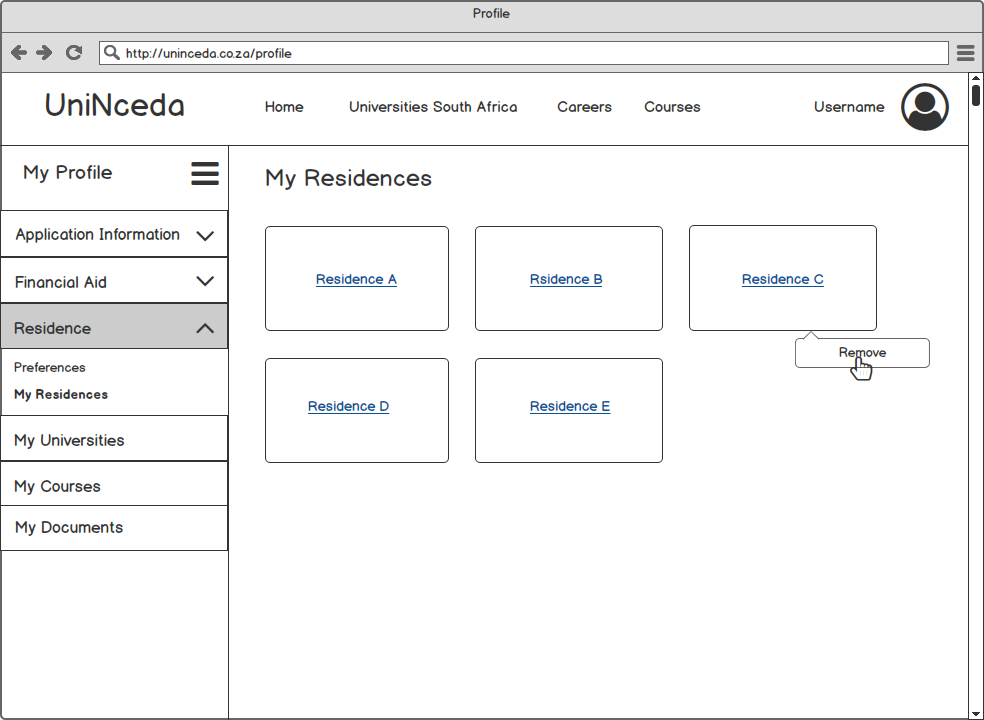
\includegraphics[scale=0.5]{ProfileResidenceResidencesRemoveResidence}
\caption{The user is able to remove a residence by right-clicking on it, then a tooltip with the text 'Remove' will appear. Clicking on this tooltip will remove the residence.}
\label{ProfileResidenceResidencesRemoveResidence}
\end{figure}

\newpage
\subsubsection{Viewing and Editing My Universities}

\setcounter{figure}{0}

\begin{figure}[H]
\centering
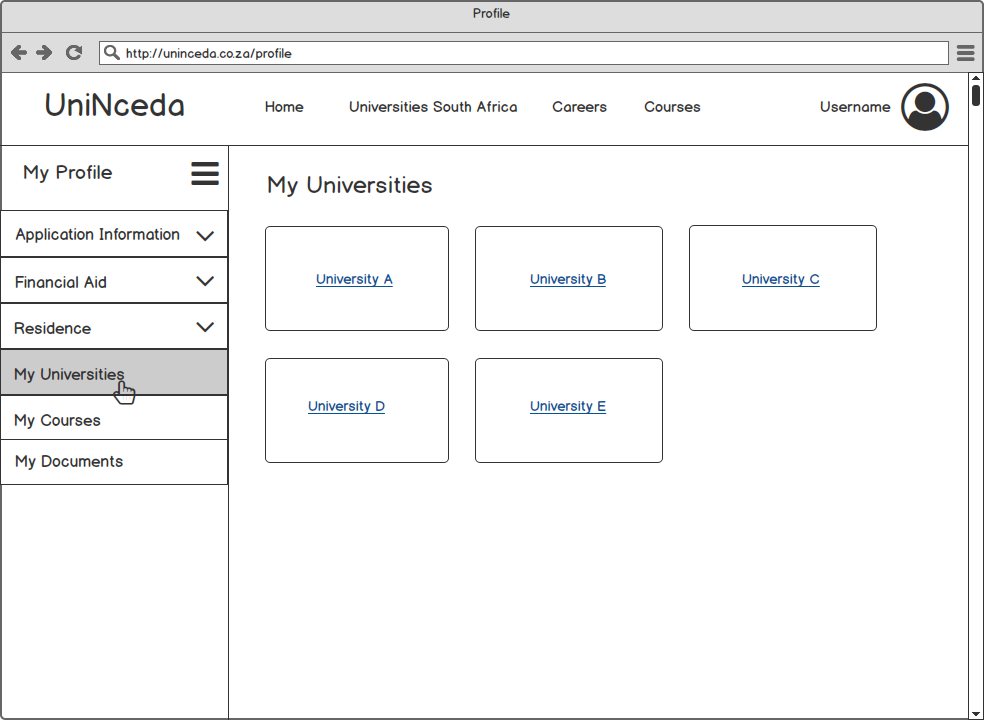
\includegraphics[scale=0.35]{ProfileMyUniversities}
\caption{Here the user is presented with a list of universities that he/she added. The user is able to click the link at any university, which will redirect the user to the page that contains the university's description on a new tab.}
\label{ProfileMyUniversities}


\vspace{1cm}

\includegraphics[scale=0.35]{ProfileMyUniversitiesRemoveUniversity}
\caption{The user is able to remove a university by right-clicking on it, then a tooltip with the text 'Remove' will appear. Clicking on this tooltip will remove the university.}
\label{ProfileMyUniversitiesRemoveUniversity}


\end{figure}

\subsubsection{Viewing and Editing My Courses}

\setcounter{figure}{0}

\begin{figure}[H]
\centering
\includegraphics[scale=0.35]{ProfileMyCourses}
\caption{Here the user is presented with a list of courses that he/she added. The user is able to click the link at any course, which will redirect the user to the page that contains the course description on a new tab.}
\label{ProfileMyCourses}


\vspace{1cm}

\includegraphics[scale=0.35]{ProfileMyCoursesRemoveCourse}
\caption{The user is able to remove a course by right-clicking on it, then a tooltip with the text 'Remove' will appear. Clicking on this tooltip will remove the course.}
\label{ProfileMyCoursesRemoveCourse}


\end{figure}

\subsubsection{Viewing uploaded documents}

\setcounter{figure}{0}

\begin{figure}[H]
\centering
\includegraphics[scale=0.35]{ProfileMyDocuments}
\caption{Here the user is presented the uploaded documents. The user can scroll down to view more documents.}
\label{ProfileMyDocuments}


\vspace{1cm}

\includegraphics[scale=0.35]{ProfileMyDocumentsPage2}
\caption{When the user scrolls down to the end of the page he/she is presented with more uploaded documents.}
\label{ProfileMyDocumentsPage2}


\end{figure}

\subsubsection{Uploading a document}
\renewcommand{\figurename}{Step}
\setcounter{figure}{0}

\begin{figure}[H]
\centering
\includegraphics[scale=0.35]{ProfileMyDocumentsBrowse}
\caption{When the user clicks the 'Browse' button, a window with a list of files pops up. In this windows the user can select the file that he/she wants to upload.}
\label{ProfileMyDocumentsBrowse}


\vspace{1cm}

\includegraphics[scale=0.35]{ProfileMyDocumentsFileSelected}
\caption{When the user clicks the 'OK' button on the windows, the file is loaded into the browser cache and the name of the file is displayed on the label.}
\label{ProfileMyDocumentsFileSelected}


\end{figure}

\begin{figure}[H]
\centering
\includegraphics[scale=0.5]{ProfileMyDocumentsUpload}
\caption{When the user clicks the 'Upload' button, the file is uploaded and stored into a database. The name and the picture of file is then displayed on the container to the left.}
\label{ProfileMyDocumentsUpload}

\end{figure}


\end{document}